\section{RESULTS}
\label{results}
\subsection{Discussions on classical ground state}
\indent \indent  We first discuss the effect of interlayer coupling semi-classically, particularly its effect on spin-wave spectrum and spin-wave velocity within the approximation by considering the terms that are quadratic in $a$'s. To do that fist we need to have an understanding about the classical ground states of model Hamiltonian given in Eq. \ref{Hamiltonian} around which spin-wave spectrum will be estimated to account for the quantum fluctuation around these classical spin configurations. Following Ref.~\cite{vijigiri2018classical}, we notice that the 3D-model Hamiltonian can also be rewritten in the following form: $H = \sum_i (h^z_i S_i^z + h^x_i S_i^x)$, where for a given spin component $S_i^\alpha$, $h^\alpha_i$ denotes the local-field component along $\alpha$ axis. The minimum energy configuration
of spins can then be obtained by aligning $S_i^\alpha$ to the negative $\alpha$ axis. We follow the same procedure that is given in Ref.~\cite{vijigiri2018classical}. We have performed numerical simulations over a lattice of dimension $16 \times 16 \times 16$ and inspected for adequate initial configurations. It is observed that in the presence of external field $K$,  all the spins would have a finite and constant value of $S_i^x$, which changes as a function
of $K$~\cite{vidal2008perturbative,vijigiri2018classical}. Therefore, the groundstate configurations
can be written as,
\begin{eqnarray}
\label{gs}
\vec{S}_i=S(\lambda_i \cos\theta \bf{e}_z + \sin\theta \bf{e}_x),
\end{eqnarray}
where $\lambda_i$ could be $\pm 1$ in tune with the ground state configurations of $H_0$ for $K=0$.  This  the configuration of $[{\lambda_i}]$ tries to take into account the other all the terms in the Hamiltonian except the Zeeman field term and a finite $\theta $ takes into account the Zeeman field induced term. The equilibrium configuration, that is, the value of $\theta_{\text{eq}}$ depends on $K$, $J_1$, $J_2$, and $J_3$. For $K=0$, we have $\theta=0$ but $\lambda$'s can still take either $\pm 1$. The $\theta$ plays the role of order parameter. From the mean-field ansatz given in Eq.~\eqref{gs}, the ground state energy of the system can be written as follows:
\begin{eqnarray}
\label{gsenergy}
E_{cl}&=&- \frac{1}{2}J_0S^4N\cos^4\theta - J_1S^2N\cos^2\theta - 2J_2S^2N\cos^2\theta \nonumber\\
&& - J_3 N S^2 \cos^2\theta - KSN \sin \theta .
\end{eqnarray}
\textcolor{red}{IN THE ABOVE EQUATION I THINK $|J_3|$ WILL APPEAR. PLEASE CHECK. BECAUSE WE CAN TAKE THE SPIN CONFIGURATIONS OF TWO NEAREST PLANE SUCH THAT THE $J_3$ BONDS HAS NO FRUSTRATION. THIS IS ALSO CONSISTENT WITH SPIN WAVE RESULTS.}
\textcolor{blue}{Now I am convinced that in the above equation $J_3$ should appear. Because when the two layers are FM/AFM way connected Eq. 9, the ansatz will have a $\pm$ signs in front of $\lambda_i$.}
\indent Minimizing $E_{cl}$ with respect to $\theta$, we obtain $\theta_C$, which minimizes the ground-state energy $E_{cl}(\theta_C)$. This ground-state energy has been compared with the $E_x=-KN$, which denotes the energy corresponding to the state where all spins are aligned along $x$-direction. For a given $J_0,J_1,J_2$, there exists a $K_c$ such that if $K\le K_c$ then $E_{cl}<E_x(\theta_C)$ with $\theta_C\le \pi/2$. One can numerically solve for $\theta_C$ and obtain the classical phase diagram~\cite{vijigiri2018classical}. \textcolor{red} {If the Hamiltonian does contain only $J_0$ and $K$, the $\theta_c$ denotes a confinement-deconfinement transition. For in this limit for $K < K_C$, the distribution of $[\lambda_i]$ minimizes four body interaction given by $J_0$. The states includes predominantly ice-rules satisfying state. In two dimension it has been found that inclusion of $J_1$ and $J_2$ increases the stability of the   deconfined phase governed by $J_0$ terms. Though inclusion of $J_1$ and $J_2$  puts certain restriction on ice-rule states, deconfined phase survives and become more stable indicating a larger value of $\theta_c$. From the mean-field decomposed classical energy expression given in Eq. \ref{gsenergy}, we find the inclusion of an antiferromagnetic (positive) $J_3$ further stabilises the deconfined phase as it adds up  directly to
the energy contribution by $J_0, J_1, J_2$.  On the other hand if $J_3$ is taken ferromagnetic then it acts apposite to the energy contribution  by $J_0, J_1, J_2$. Thus it destabilizes the deconfined phase and reduces the value of $\theta_c$.}  \\
\indent  The classical ground-state has finite degeneracy in the presence of $J_0, J_1$, and $J_2$ which remains unchanged after inclusion of interlayer coupling $J_3$. For finite interlayer coupling, that is, $J_3>0$ $J_1=J_2=0$, the degeneracy is still $2^{N_xN_y+1}$  and for $J_2=0$, the degeneracy is $2^{N_x+N_y}$. For both $J_1$ and $J_2$ nonzero, the degeneracy is reduced to four as in the case of 2D case~\cite{vijigiri2018classical}. For large $K>Kc$, all the spins get aligned along the $x$-axis corresponding to $\theta_c=\pi/2$. The degeneracy of 3-dimensional system follows directly the degeneracy of a any  two dimensional plane for ferromagnetic and anti-ferromagnetic interlayer coupling. This is seen in the simulations where the specific heat shows an anomalous peak whose height is proportional to this degeneracy. \textcolor{red}{The degeneracy of three dimensional system is not straightforward to calculate for a disordered configurations of interlayer coupling.  In the disorder case, the spin-configuration of two nearest-neighbour two dimensional plane are frustrated. However it could very much happen that while the spin configurations of any two-dimensional planes are frustrated, there are many degenerate configurations which all are frustrated but have the same energy. Interestingly it may also happen within this degenerate manifold of frustrated ground state configuration a certain two dimensional plane is not frustrated. Thus the exact determination of effect of disordered interlayer coupling on the degeneracy is very subtle. However later we will observe that the specific heat shows a reduced anomalous  peak at lower temperature which asserts the fact that some residual degeneracy survives.}
\subsection{Linear spin-wave theory}
\indent \indent In the previous section we have found that the classical ground-state spin configuration  obtained is  dependent on $\theta$ implying that we can define a local axis represented by $x^{\prime} (z^{\prime})$. This $(x^{\prime}, z^{\prime})$ is obtained from $(x,z)$ by a rotation by angle $\theta$ around $y$-axis. The spin operators in prime co-ordinate is defined by $\bf{S}^{x^\prime}_r = s - \bf{a}^\dagger_r\bf{a}_r,  \hspace{2mm} \bf{S}^{z^\prime}_r = \sqrt{s/2}(\bf{a}^\dagger_r + \bf{a}_r) $ within large $\bf{S}$ approximation \cite{Ref}. \textcolor{red}{Here $ \bf{a}^{\dagger}$ denotes the creation of magnon operators which are defined along the  directions of alignment of local $z^{\prime}$-axis.}  To make use of this definition we have to rotate the local axis to the global co-ordinate systems, which is given as,
\begin{eqnarray}
\label{rotation}
\bf{S}^x_r &=& \bf{S}^{x^\prime}_r \cos\lambda_i\theta - \bf{S}^{z^\prime}_r \sin\lambda_i\theta, \\
\label{rotation1}
\bf{S}^z_r &=& \bf{S}^{x^\prime}_r \sin\lambda_i\theta + \bf{S}^{z^\prime}_r \cos\lambda_i\theta.
\end{eqnarray}
\begin{figure*}
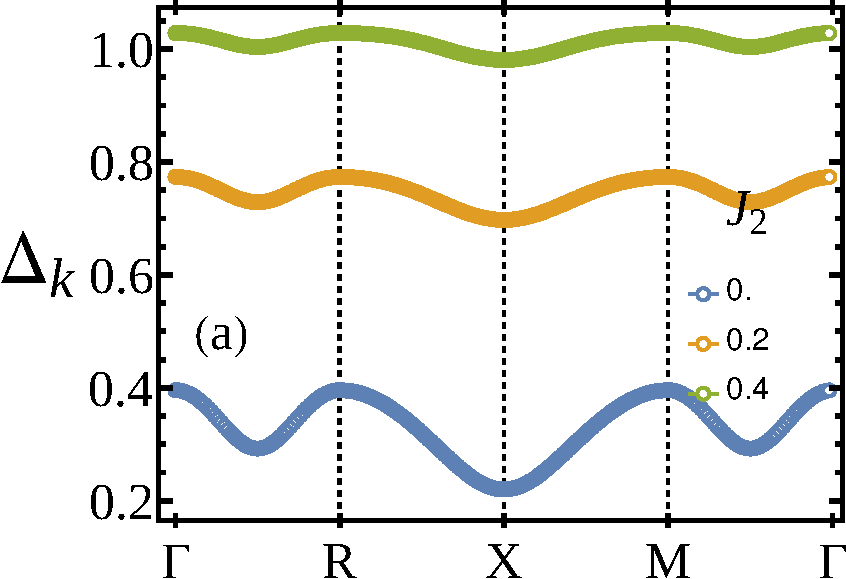
\includegraphics[width=5cm,height=3.5cm,valign=t]{figures/sw_1.pdf}
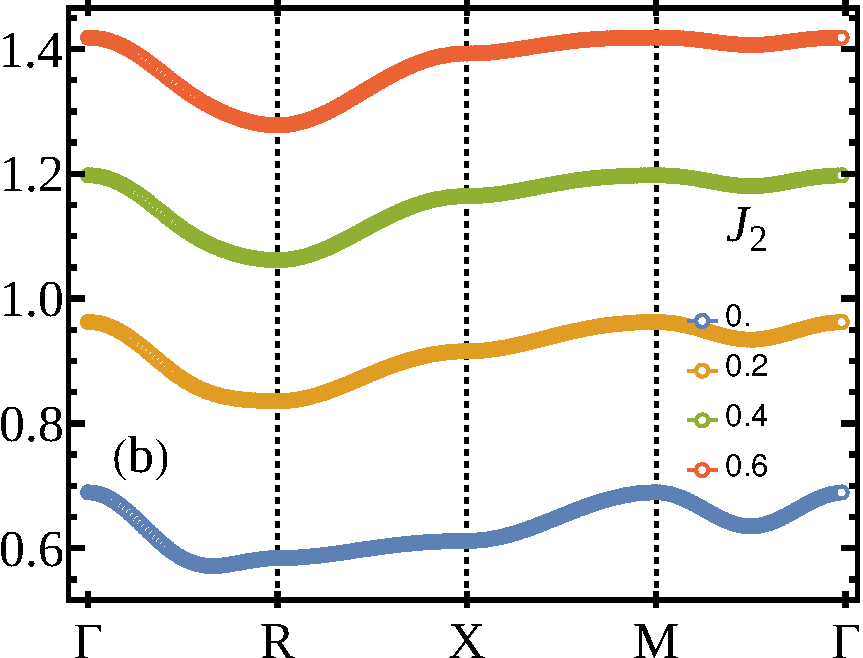
\includegraphics[width=4.2cm,height=3.5cm,valign=t]{figures/sw_2.pdf}
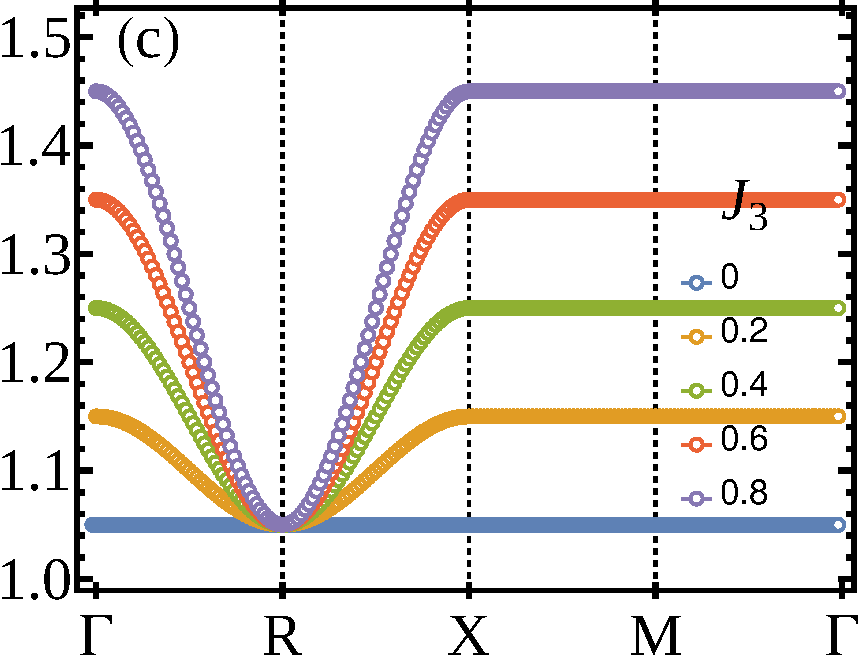
\includegraphics[width=4.2cm,height=3.5cm,valign=t]{figures/sw_3.pdf}
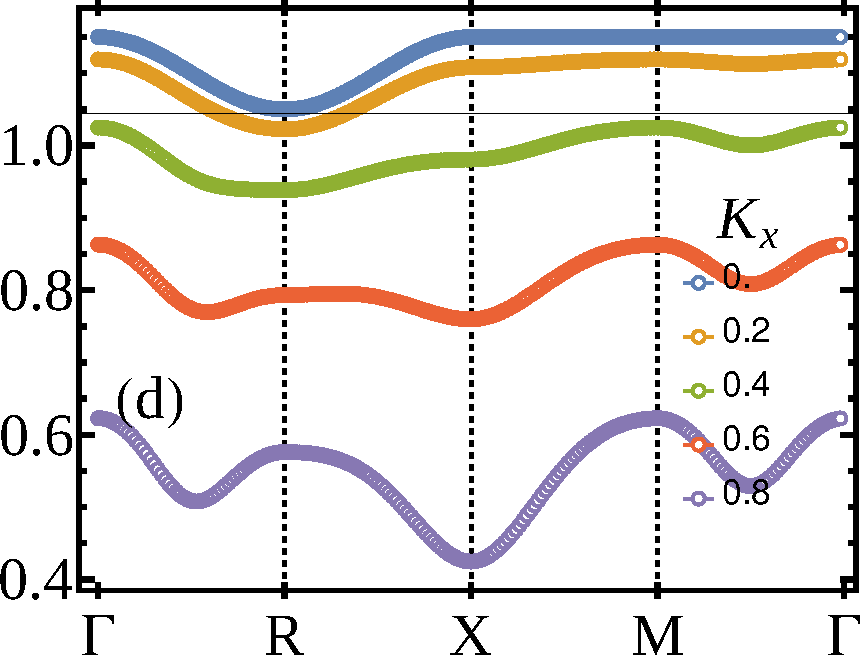
\includegraphics[width=4.2cm,height=3.5cm,valign=t]{figures/sw_4.pdf}
\caption{\label{square} Plot showing the dispersion in the high-field case where quadratic behavior slowly converges to a linear behavior at the
second-order critical line given by $K = 2sJ_1 + \frac{21}{8}sJ_2+2s|J_3|$. The spectrum is plotted for various values of $J_2$, the rest of the parameters used in plot (a) are:
$J_3 = 0$, $K = 0.5$, $J_1 = 0.5$,  $J_0 = 1.0$. Similarly for plot (b),  $J_3 = 0.2$, $K = 0.5$, $J_1 = 0.5$, $J_0 = 1.0$. And for plot (c), $J_3 = 0.8$, $K = 0.5$, $J_1 = 0.5$, , $J_0 = 1.0$. The various symmetry point used in the above figure is as follows: $\Gamma$ =
$(0, 0, 0)$, $R$ = $(\pi, \pi, \pi)$, $X = (0, \pi, 0)$, and $M = (\pi, \pi, 0)$. \textcolor{blue}{There are some problems with the labelling. Label (c) is missing. I think the plot which is labelled as (b) should be (d). Which is labelled as (d) should be (c) and which is labelled as (a) in the lower left panel is (b). By this we can only attribute the abrupt or completely different spin-wave spectrum shown in the right upper panel. This is for maximum $J_3$ and this shows minima around (R) point. also from the input file sw$_1$.pdf has been used twice. Also in the y-axis $\Delta_k$ has been used. Is it same as $E_k$ or not?}}
\label{highfield}
\end{figure*}

%\begin{eqnarray}
%\label{hptransform}
%\bf{S}^{x^\prime}_r = s - \bf{a}^\dagger_r\bf{a}_r,  \hspace{2mm} \bf{S}^{z^\prime}_r = %\sqrt{s/2}(\bf{a}^\dagger_r + \bf{a}_r).
%\end{eqnarray}
\indent Once  we substitute the above definitions in to the Hamiltonian we obtain the so called spin-wave Hamiltonian. We note that spin-wave Hamiltonian contain quadratic term along with quatric and cubic term. In the following we only retain the terms upto quadratic to make further progress.\\

\subsubsection{\textcolor{blue}{Discussion in the small field limit}}
\textcolor{blue}{Previously in the two dimensional case we have found that in the small field limit, the spin wave spectrum does not cause any order from disorder transition. The macroscopically degenerate ground state manifold have identical ground state energy under quantum fluctuation in quadratic approximation. This happens due to the presence of macroscopic conserved quantities discussed previously \cite{vijigiri2018classical}Now some comments about three dimensional case will be enligtening and is a very important point. What we all need is to tame few $N_x \times N_y \times N_z$ systems and calculate the ground state energy and check whether there are some order from disorder transition. I guesst that there will be some transition and this will be one of the main results. }
\subsubsection{High-field limit, $K \gg J_0,J_1,J_2$ \& $\theta_0=\pi/2$}
\indent \indent The groundstate in this limit is a trivial one with all the spins pointing towards the $x$-axis. To obtain the magnon-spectrum and to check the stability of the classical groundstates, the Holstein-Primakoff transformation Eq.~\eqref{hptransform} is substituted into the classical version of the  Hamiltonian~\ref{Hamiltonian} with the groundstate Eq.~\eqref{gs} now being explicitly embedded into it. Since in the high-field case we invoke the translation invariance of the spin-configurations, we then can Fourier transform the $a_i$ variables to $a_k$ as $a_i=\frac{1}{N}\sum_{\vec{k}}a_{\vec{k}}\exp({-i\vec{k}\cdot\vec{r}})$. Substituting the transformed boson operators into the above equation yields a Hamiltonian of various orders in $a$. Within quadratic approximation we neglect the higher order terms beyond second order, the Hamiltonian then is given by,
\begin{eqnarray}
\mathcal{H}&=&N\sum\limits_{k}\bigg[\xi_ka_ka^\dagger_k + \frac{\gamma_k}{2}(a_ka_{-k} + a^\dagger_k a^\dagger_k)\bigg] +  C_0 + \mathcal{O}(a^3)\nonumber \\
&&+ \mathcal{O}(a^4),
\end{eqnarray}
where $C_0=KSN$ and is the classical energy upon which the terms within the bracket has the information of the first dispersion in $k$-space, given by $\xi_k$. The $\xi_k$ and $\gamma_k$ is given below as,
\begin{eqnarray}
\xi_k&=&\gamma_k + K -\frac{SJ_2}{8},\\
\label{pk}
\quad \gamma_k &=&\frac{-s}{4}\big[J_2(2 p_k^2 -1) - 4(J_1+J_2)p_k\nonumber \\
&&+ 4|J_3|\cos(k_z)\big],
\end{eqnarray}
where $p_k=\cos(k_x+k_y)\cos(k_x-k_y)$. Now, the Hamiltonian is easily diagonalizable and upon doing that we obtain the eigen energies of the magnon spectra as given by,
\begin{eqnarray}
\label{dispersion}
E_k&=& \sqrt{\xi^2_k - \gamma_k^2}.
\end{eqnarray}
\indent In the Fig.~\ref{highfield} we show the spectrum plotted for parameters $J_1=0.2, K=1.0$ and varying $J_2$ from $0.1$ to $0.5$ \textcolor{red}{This is not consistent with what is said in Fig. \ref{square}}. To qualitatively decipher the linearity seen in the dispersion curves obtained for $J_2=8/21$ we find the spectrum by extracting the low-energy behavior around the minima, that is, $X$ (or $R$) high-symmetry point. We consider the following approximation $(k_x=-\pi/2 + \delta_x, k_y=\pi/2 + \delta_y, k_z=\pi + \delta_z)$ around $R$. Substituting these in Eq.~\eqref{dispersion} and expanding the terms $\gamma_k, p_k$, we get,
\begin{eqnarray}
\label{linearspectrum}
E_{\vec{\delta}}=\tilde{K}_1^{1/2}\sqrt{\tilde{K}_2 + 4(J_1 + 2J_2+|J_3|)|\vec{\delta}|^2},
\end{eqnarray}
here, $\tilde{K}_1=K-\frac{sJ_2}{8}$, $\tilde{K}_2=(K-2sJ_1-\frac{21}{8}sJ_2+2s|J_3|)$. From the Eq.~\eqref{linearspectrum} we can see that for all the values of $J_{1,2}, K$ the spectrum remains gapped with low-energy quadratic behavior in the dispersion curves except at the second-order transition point as obtained by $K_c=2sJ_1 + 21/8J_2+2s|J_3|$ \textcolor{blue}{This is also consistent with the results of classical analysis that $k_c$ increases with $J_3$, the deconfined phase gets more stable. But this $K_c$ is unusually high}. The spectrum at this point becomes linear and gapless, indicating a possible signature of with the underlying features of the groundstate for higher $J_2$, which is the antiferroelectric case. This also shows that the transition for smaller values of $J_2$ the system behaves quite differently from the one with relatively higher values of $J_2$. This can be attributed to the fact that the gapped spectrum is protecting the degeneracy in the groundstate manifold in the absence of dipole-dipole interaction $J_2$, with the excitations being gapped and discrete. \textcolor{red}{When $J_2$ is increased and approaches the antiferroelectric ordered state, the spin-wave spectrum becomes linear and gapless as expected.BUT FROM THE FIGURE 2. INCREASE OF $J_2$ SEEMS TO MAKE THE SPECTRUM MORE OR MORE FLATTER. THIS IS BECAUSE OF $J_3$ OR NOT? IT SEEMS THERE IS SOME ESSENTIAL DIFFERENCES BETWEEN TWO DIMENSION AND THREE DIMENSONS AS FAR AS THE ACTION OF $J_2$ IS CONSIDERED. IN TWO DIMENSION INCREASE OF $J_2$ MAKES THE SPECTRUM LINEAR BUT IN THREE DIMENSIONS IT IS BECOMING MORE GAPPED OUT DUE TO THE PRESENCE OF $J_3$.} And as one increases the value of $J_2$ further we see that the $\tilde{K}_2$ changes to negative in sign where the spectrum becomes imaginary~\eqref{linearspectrum}. The same can be deciphered from the Fig.~\ref{highfield} shown in dotted lines near the $X(R)$ high-symmetry points where there are no states available with the gap $\Delta(k)$ being undefined. It is to be noted that for sufficiently large $J_2$ one needs to perform the SW analysis on a different groundstate. Importantly, from Eq.~\ref{linearspectrum}, we can see that the spin-wave velocity is independent of the nature of the coupling. Since,
\begin{eqnarray}
\frac{\partial(E_{\vec{\delta}})}{\partial{\vec{\delta}}}\propto |J_3\vec{\delta}|\tilde{K}_1^{1/2}\sqrt{\tilde{K}_2 + 4(J_1 + 2J_2+|J_3|)|\vec{\delta}|^2}.
\end{eqnarray}
\indent\textcolor{red}{The indistinguishability of the spin-wave velocity can be understood as follows: Let us consider a single layer, in a ground state of $J_0$, where each plaquette can take up to 8 different configurations with the same energy (four of them are shown in Fig.~\ref{rho_ice_rules}(a)). Now, if we pick any one of the eight states we see there exists one high-energy (from the rest of the seven states) state that appears at finite temperatures or fields. And, six of the low-energy choice where the system can exist at low-temperatures (from the remaining six other choices). Similarly, we do the same analysis for the AFM case and we see the same number of choices are available even for that case. That is even for AFM coupling there exists six low-energy choices and one high-energy choice the system can exist. Hence, we note that this choice of states is independent of the nature of the coupling, i.e, it does not distinguish whether the coupling is AFM or FM. This is reflected in the spin-wave spectrum and thus we obtain identical spin-wave velocity.THE ABOVE ARGUMENT DOES NOT LOOKS CONVINCING. IT HAS TO DO WITH SOME SYMMETRY SUCH THAT IN EQ. \ref{pk} ONLY MOD $J_3$ APPEARS. THIS IS SOMETHING TO $Z_2$ SYMMETRY. now i doubt whether the sign of $J_3$ as taken in Eq. \ref{gsenergy} is taken correctly.}\\
\indent
\textcolor{blue}{COMMENTS:  The results on classical ground states by estimating $K_c$ for various parameters and comparing with the $K_c$ obtained from spin-wave analysis and further comparing with $K_c$ obtained from the monte-carlo simulations of correlation function(as given in Eq. \ref{imag-time-correlation}) will give a very nice way to understand the effect of quantum fluctuation and role of FM, AFM or disordered coupling. This is in our hand. All we need to do is take a consistent choice of parameter values in all the three analysis. This will be taken as an important motivation to study different methods, in the abstract we can also write that we determine the $K_c$.}
%%%%%%%%%%%%%%%%%%%%%%%%%%%%%%%%%%%%%%%%%%
\subsection{Imaginary-time quantum Monte Carlo}
\indent \indent  First, we consider the confinement-deconfinement transition (CDT) where $J_2=0$. We vary the external field for various interlayer couplings, and calculate the imaginary-time correlation $c_\tau$ as a function of $\tau$, as shown in Fig.~\ref{imag-time-correlation}. Similarly, in the next section, we provide the results for the order parameter $P,\rho$ and specific heat $C$ for $J_2\neq 0$ where the material is believed to host the AFM phase.
%%%%%%%%%%%%%%%%%%%%%%%%%%%%%%%%%%%%%%%%%%%%%%%%%%%%%%%%%%%%%%%%%
                % CDT transition
%%%%%%%%%%%%%%%%%%%%%%%%%%%%%%%%%%%%%%%%%%%%%%%%%%%%%%%%%%%%%%%%%
\begin{figure}[t!]
\centering
\hspace{-0.1cm}
%\includegraphics[width=.5\textwidth]{order_param.pdf}
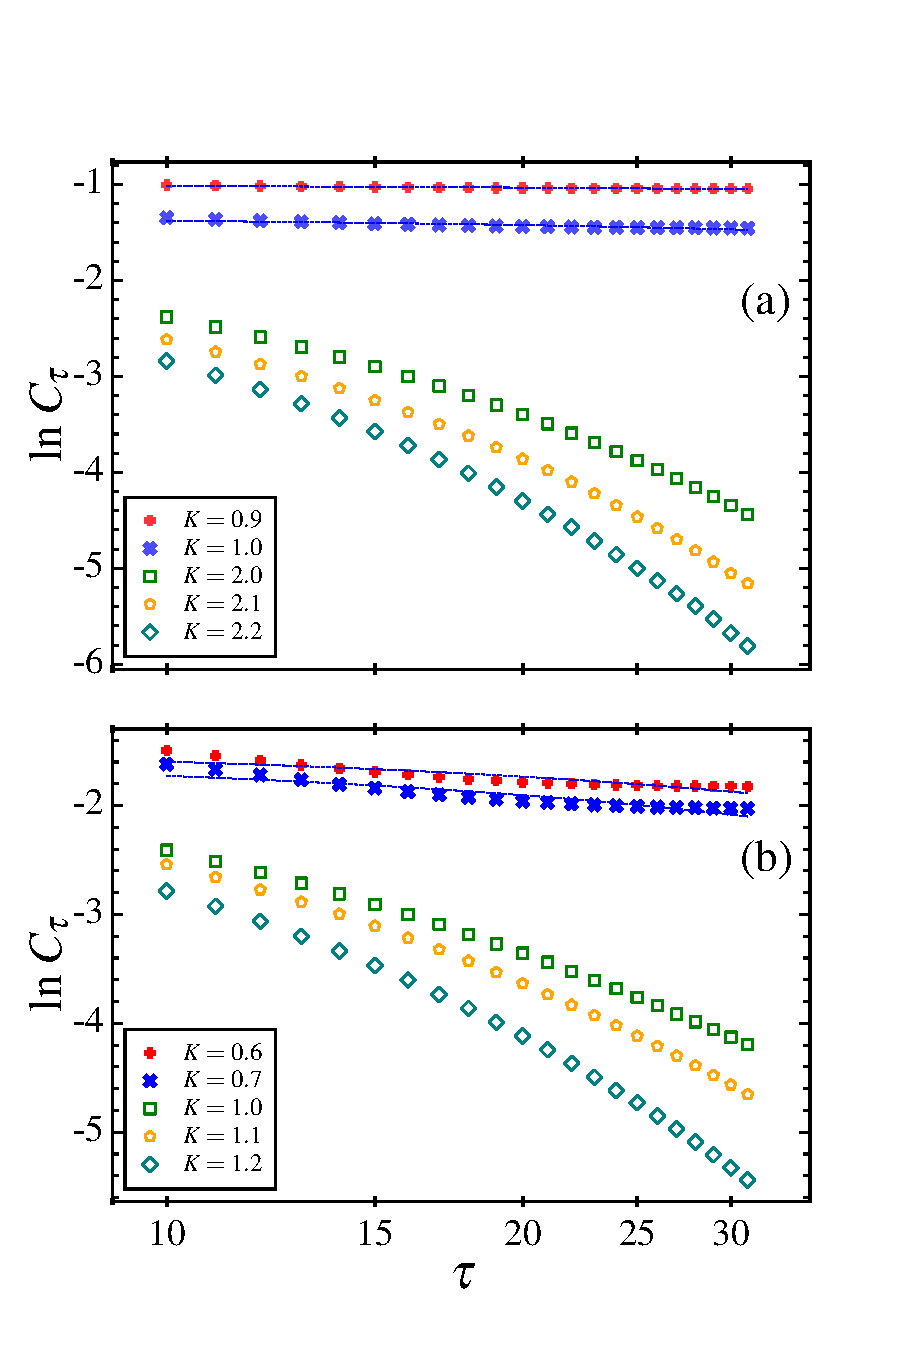
\includegraphics[width=8.0cm,height=12.0cm]{figures/corr_plot_.pdf}
\caption{Plots showing the variation of the correlation function $c_{\tau}$ along the imaginary-time axis as estimated for different values of field strength. $J_0=J_1=1.0$ is used in all the figures here. (a) Corresponds to the case where the strength of the interlayer coupling $J_3=0.1$ with a critical value of $K_c=1.63$.  Similarly, (b) for $J_3=0.3$. We see that the correlation function decays according to the power-law for low-field values, that is, for $K=0.6,0.7$ ($K<K_c=0.94$) and then an exponential decay for $K=1.0,1.1,1.2$ ($K>K_c$). \textcolor{blue}{here we see that as we increase the value of $J_3$, value of $K_c$ decreases. This means the deconfined phase is destabilized as we increase the value of $J_3$, this is against the classical analysis which seems to suggest that $K_c$ increases as we increase $J_3$. However the results could be all correct because in the quantum simulation proper account of three dimensional structure is considered and the fluctuation of spins at nearest neighbour plane helps to confine the protons easily, more to thin. Physically we need to think how the increase of $J_3$ helps in confining, or help assisting $K$ in confining the protons.  }} %\mandal{What is the Kc..is there any numerical values for a given set of parameter. Also a natural question arises to take the $J_3$ limit zero. Naturally one would be interested to know whether the interlayer coupling increases or decrease the correlation value. } \color{blue}{Edited accordingly: VIKAS}}\label{order_param}
\label{imag-time-correlation}
\end{figure}
\subsubsection{Confinement-deconfinement transition}
\indent \indent In Fig.~\ref{imag-time-correlation}(a-b), we plot $\log c_\tau$ versus $\tau$ for various values of field strengths. The plots are shown for $J_3$ where the coupling is taken as disordered type. We see that when the field strength is below a critical field of $K_c=1.63$ (Fig.~\ref{imag-time-correlation}), the $\log c_\tau$ curve starts deviating from the power law decay (a behavior corresponding to a deconfined phase~\cite{chern2014gauge}). The functional form we fit is given by $c_\tau=r^{-n}\exp{r/r_0}$ (here, $n\sim 0.61$), that is, a behavior intermediate between a power law and exponential decay. We distinguish both the phases by the fact that in the paraelectric phase the behavior one expects is purely exponential decay (cases where $K=2.0,2.1,2.2$ in Fig.~\ref{imag-time-correlation}(a)). Similarly, in Fig.~\ref{imag-time-correlation}(b) where the strength of $J_3$ is now higher and is equal to 0.3, we see the function $c_\tau$ shows a lesser amount of long-range correlation for $K=0.6,0.7$ ($K<K_c$) decaying slowly away from the power-law $\sim$ 1/$r^{\eta-d/2+\nu}$ compared to Fig.~\ref{imag-time-correlation}(a). This may be due to the reason that the quantum fluctuations in higher dimensions are much more pronounced leading to such a behavior.  However, intuitively, when the field strength is further increased we see that the $c_\tau$ deviates more and more away from the power-law (see the blue dot curve in Fig.~\ref{imag-time-correlation}) as it decays according to the exponential law corresponding to a confined phase. The critical point for $J_3=0.1$ is $K_c=1.63$ and similarly for $J_3=0.3$ is $K_c=0.94$.  \\
\begin{figure*}[t!]
\centering
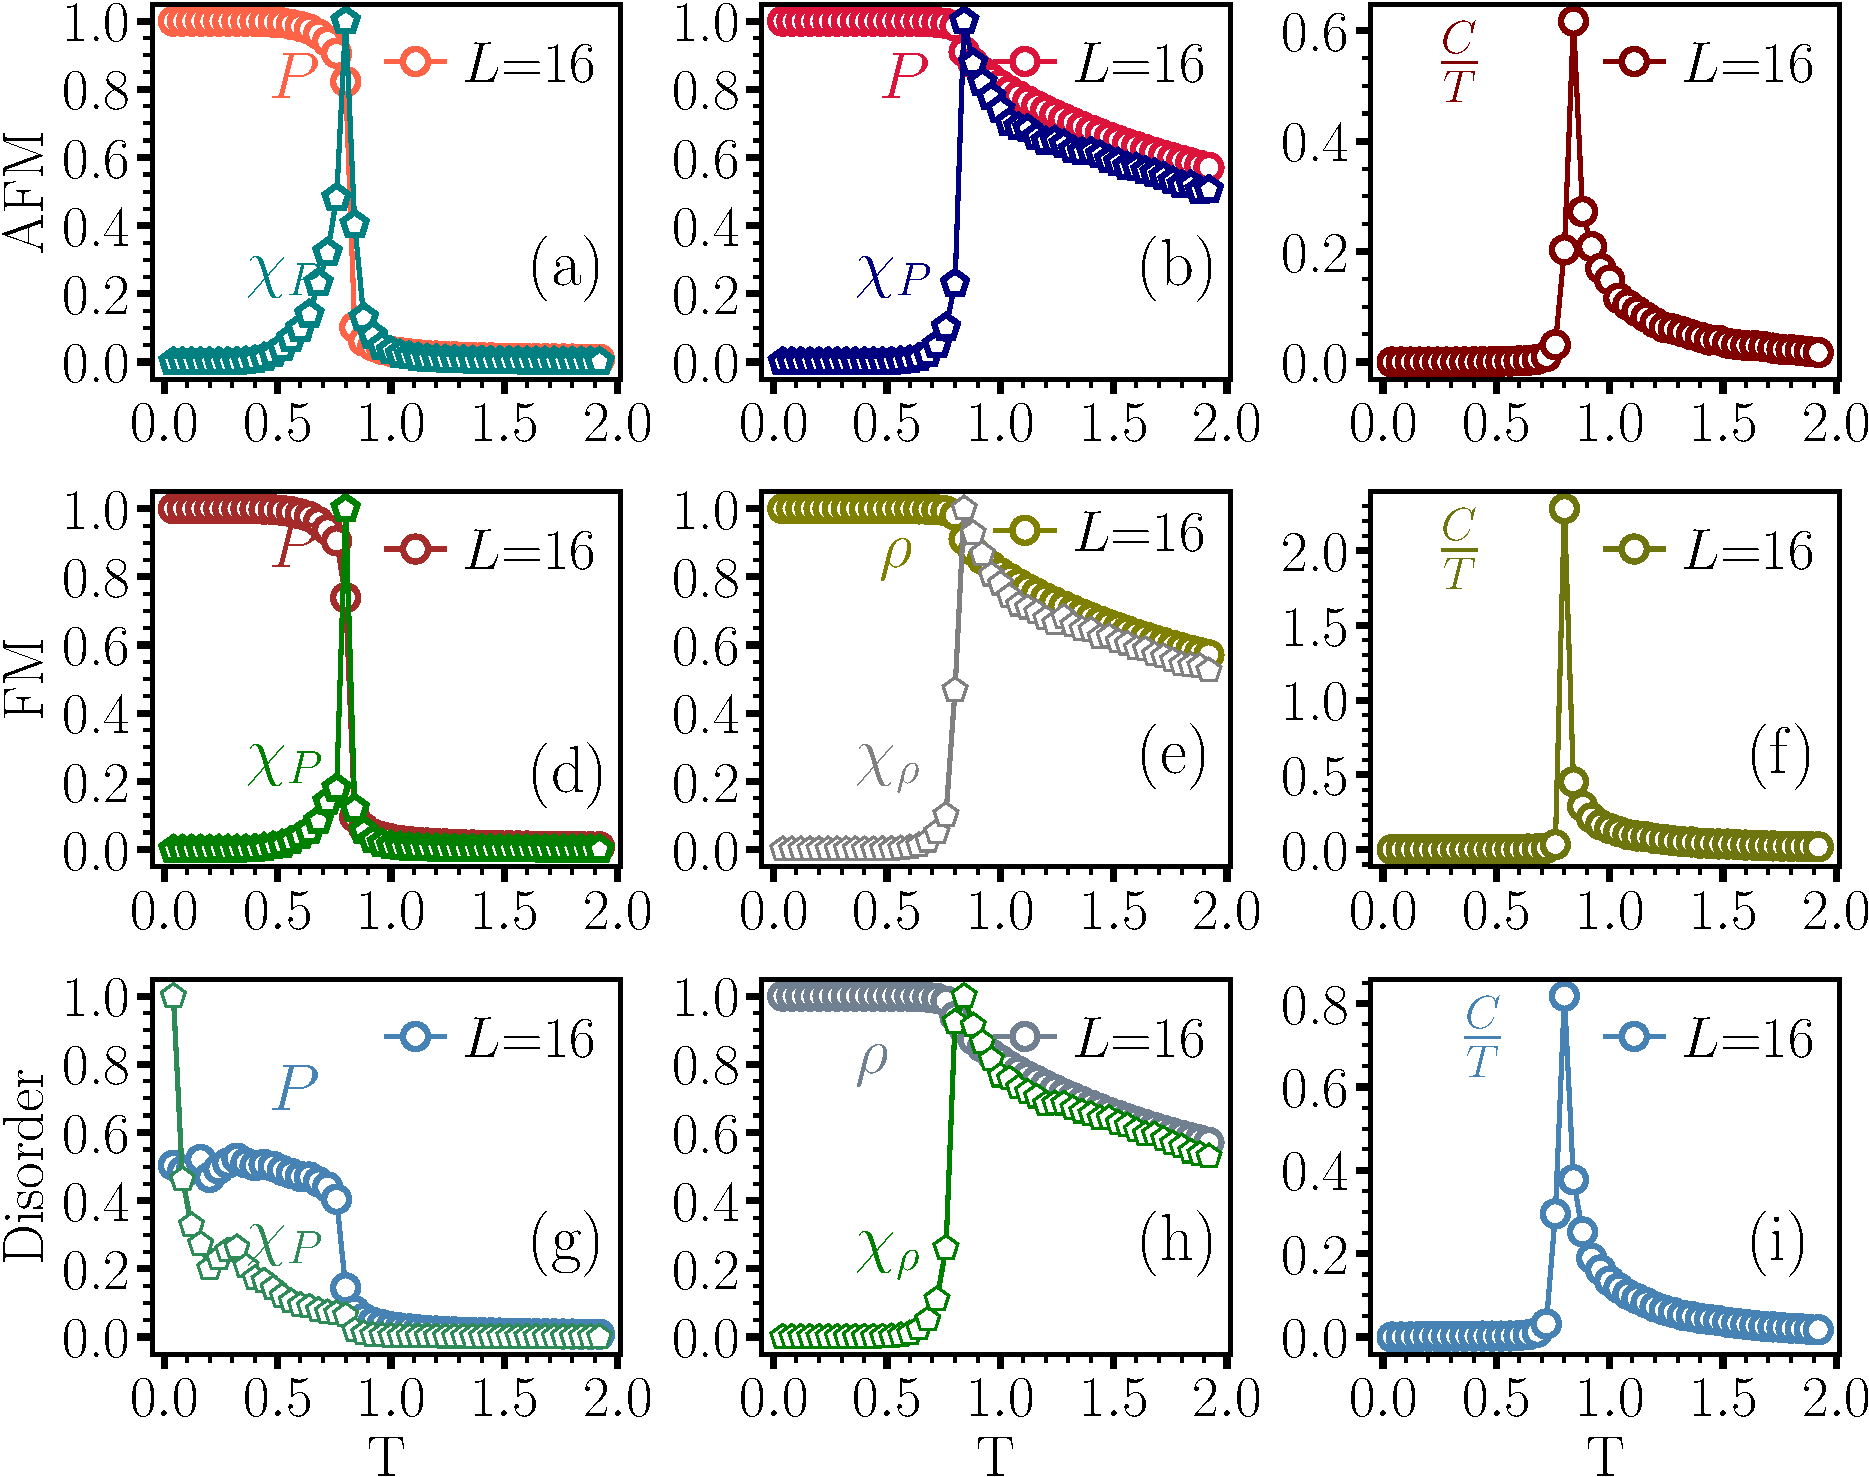
\includegraphics[width=1.0\textwidth]{figures/all_T_0.5_0.05_0.03_16_1_8.pdf}
%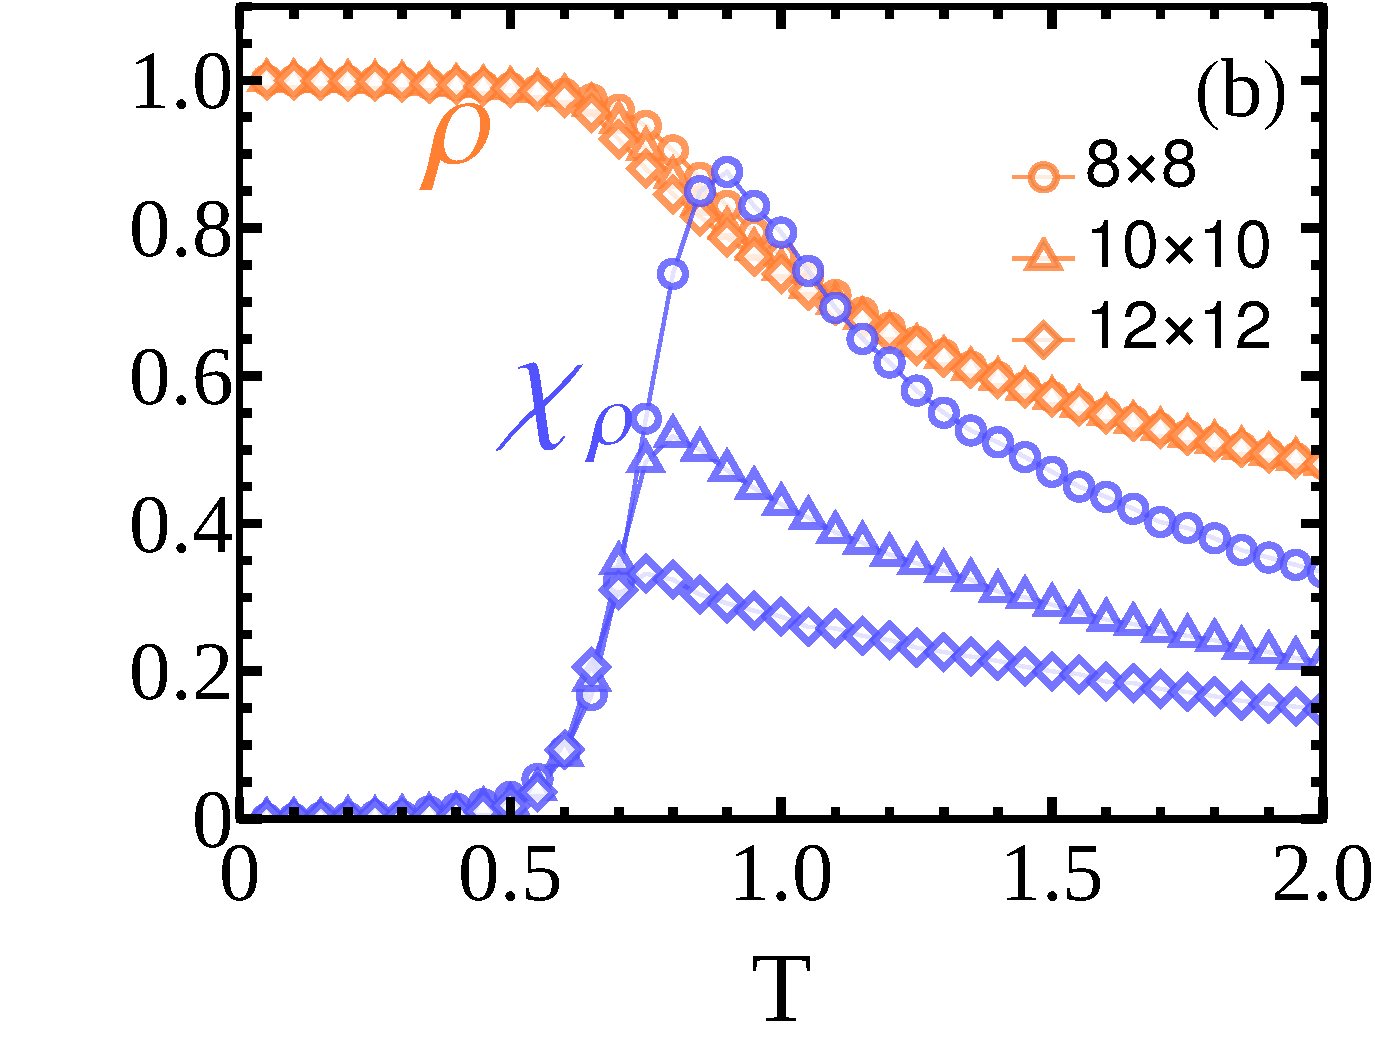
\includegraphics[width=0.3\textwidth]{figures/AFM2.pdf}
%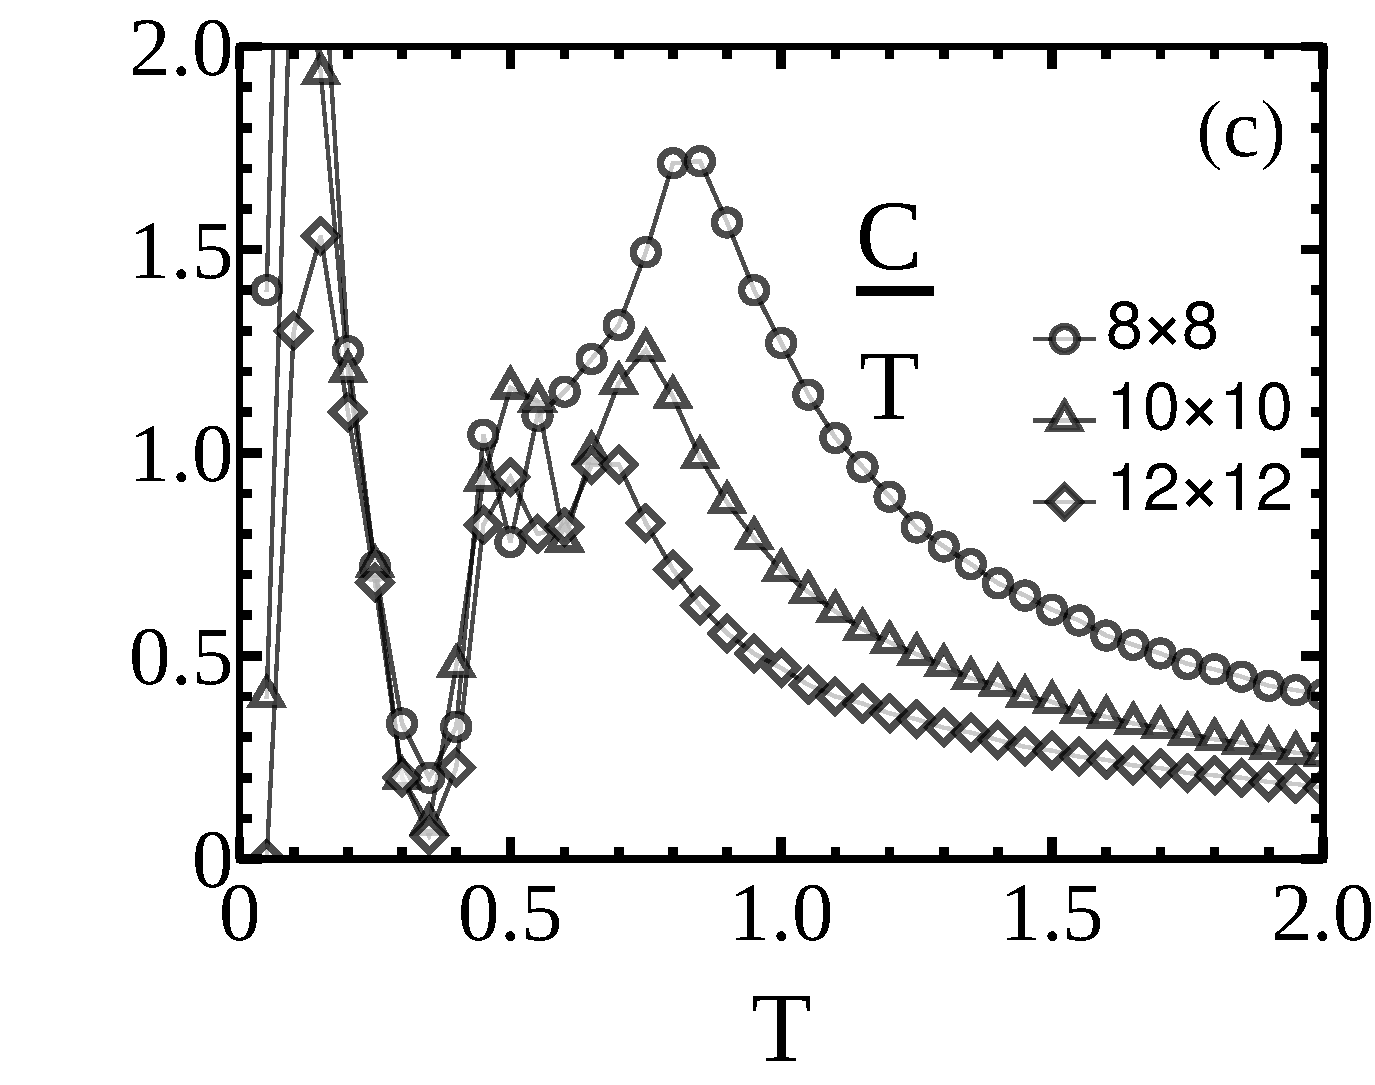
\includegraphics[width=0.3\textwidth]{figures/AFM3.pdf}
%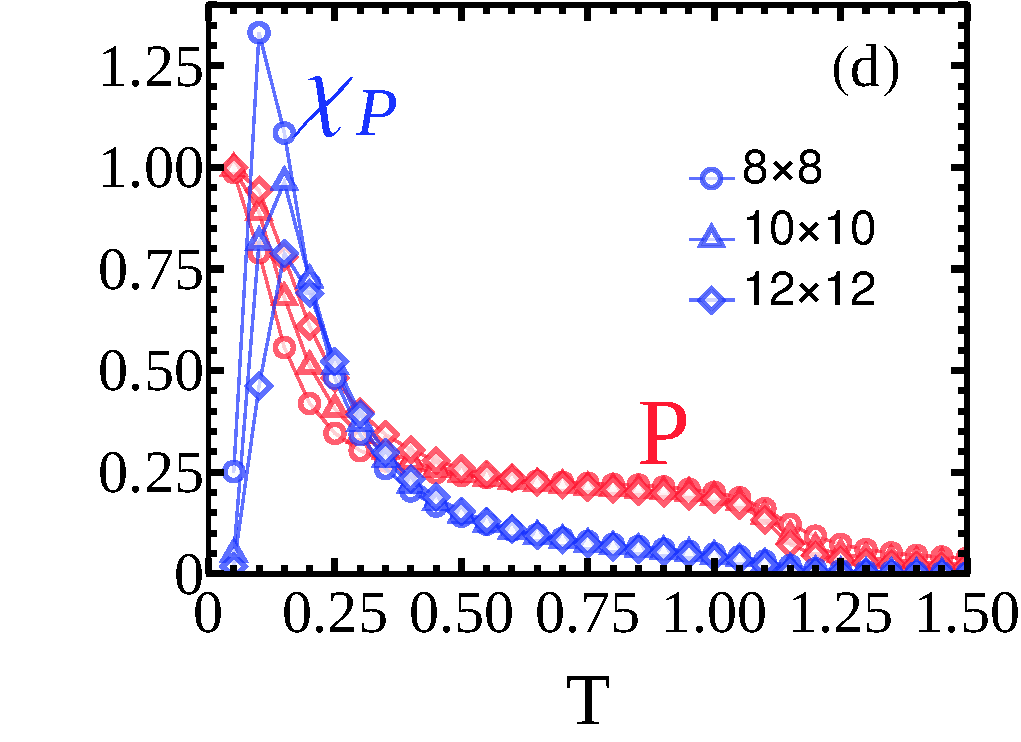
\includegraphics[width=0.33\textwidth]{figures/FM1.pdf}
%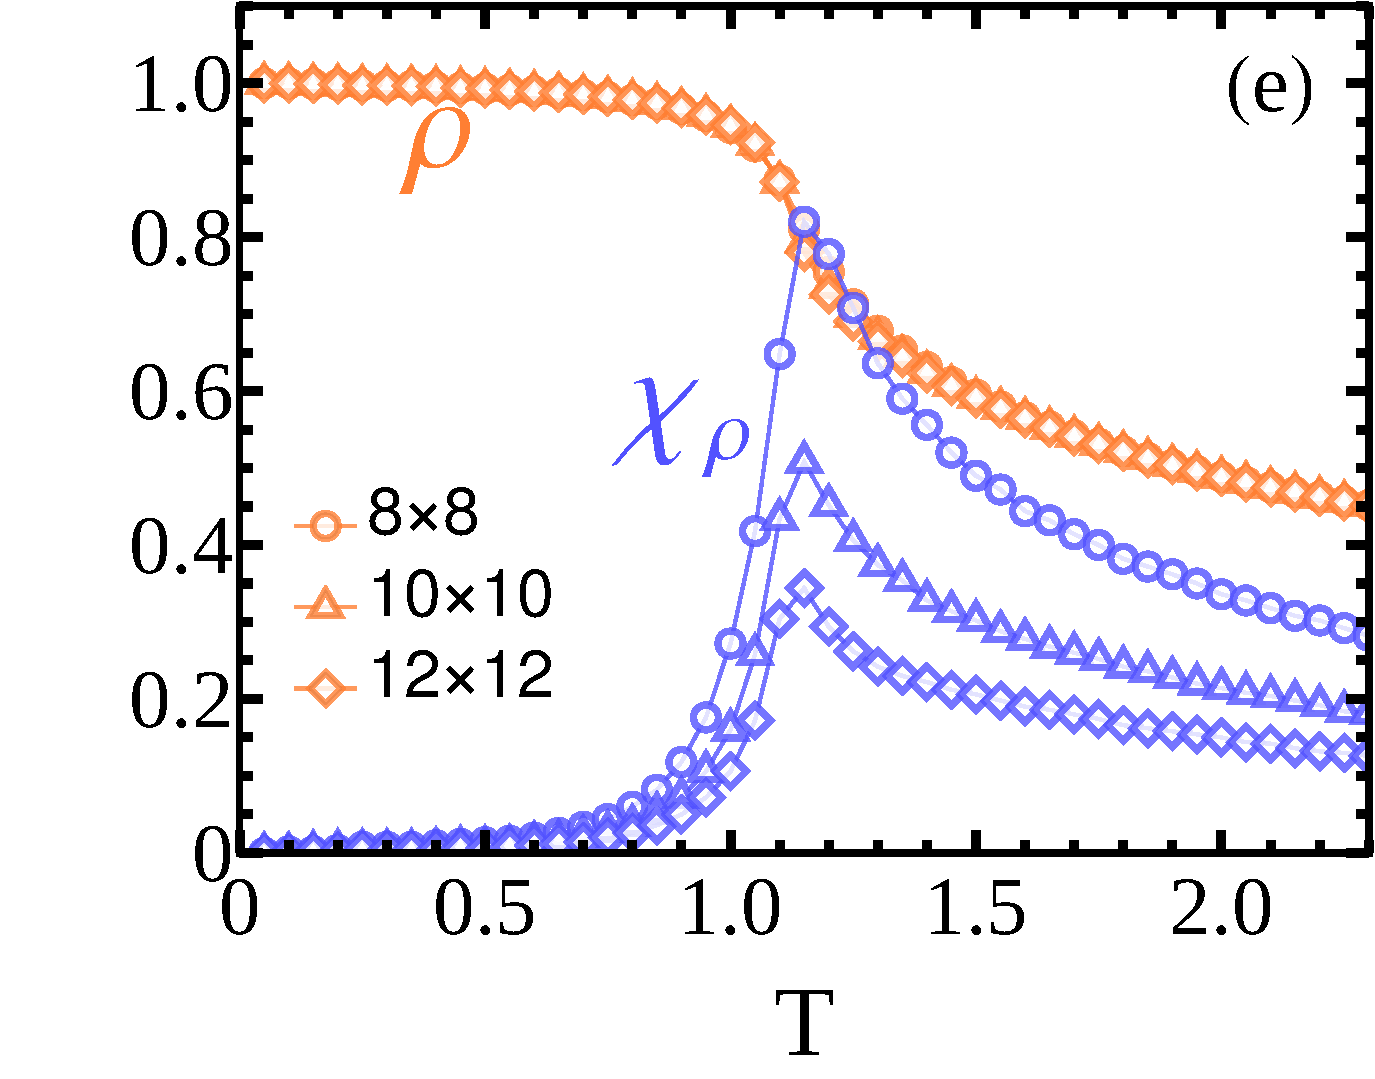
\includegraphics[width=0.3\textwidth]{figures/FM2.pdf}
%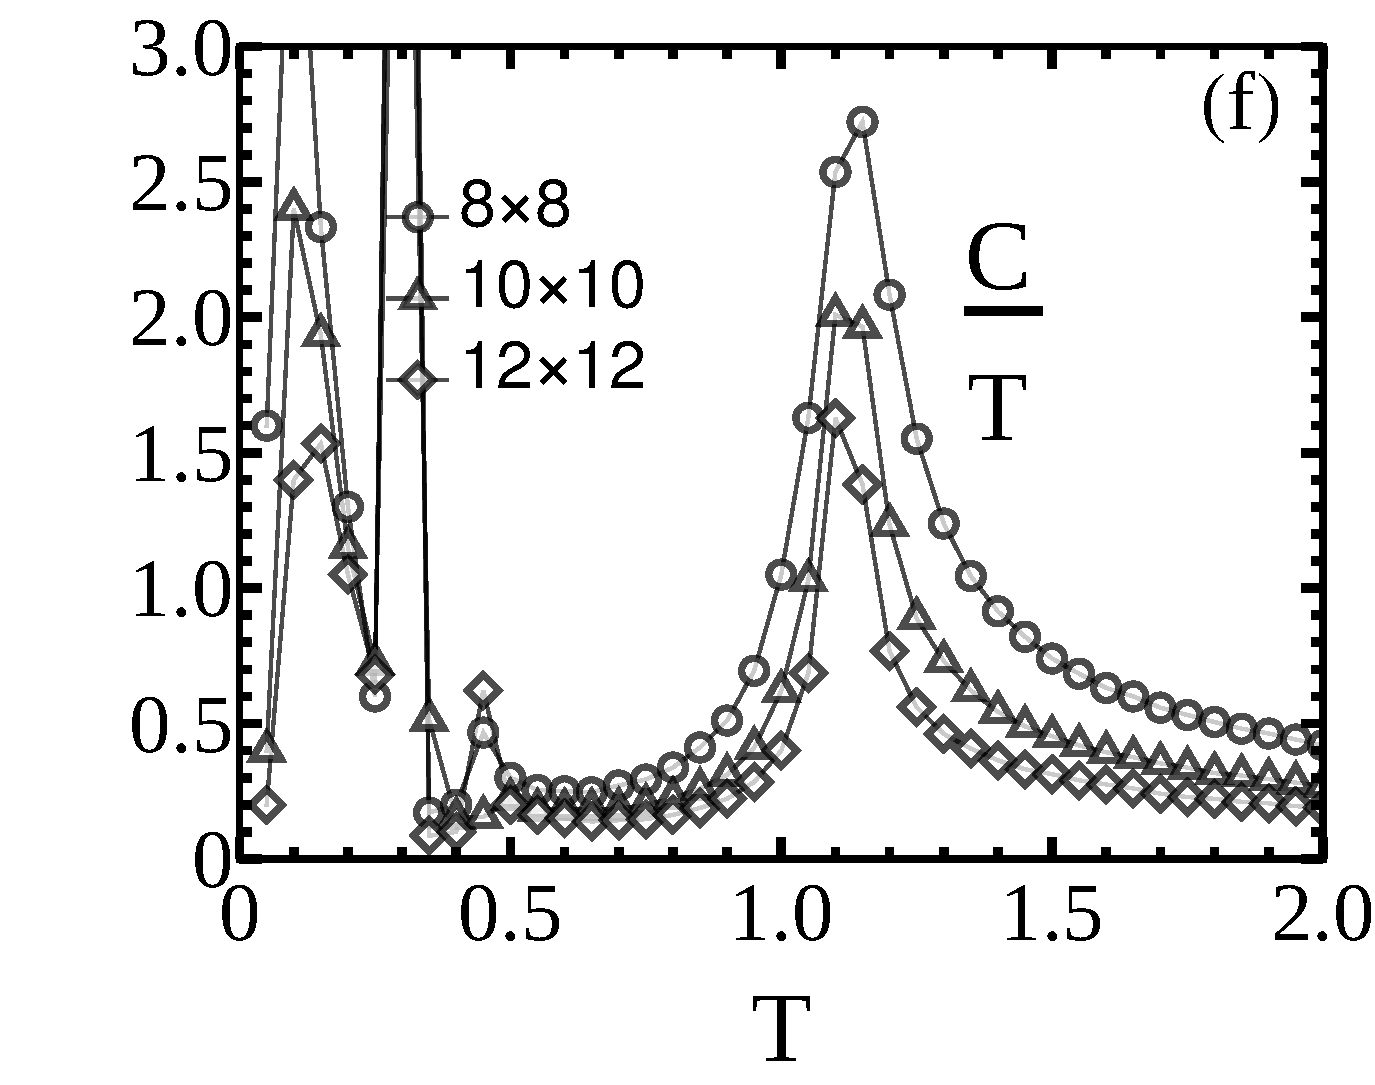
\includegraphics[width=0.31\textwidth]{figures/FM3.pdf}
%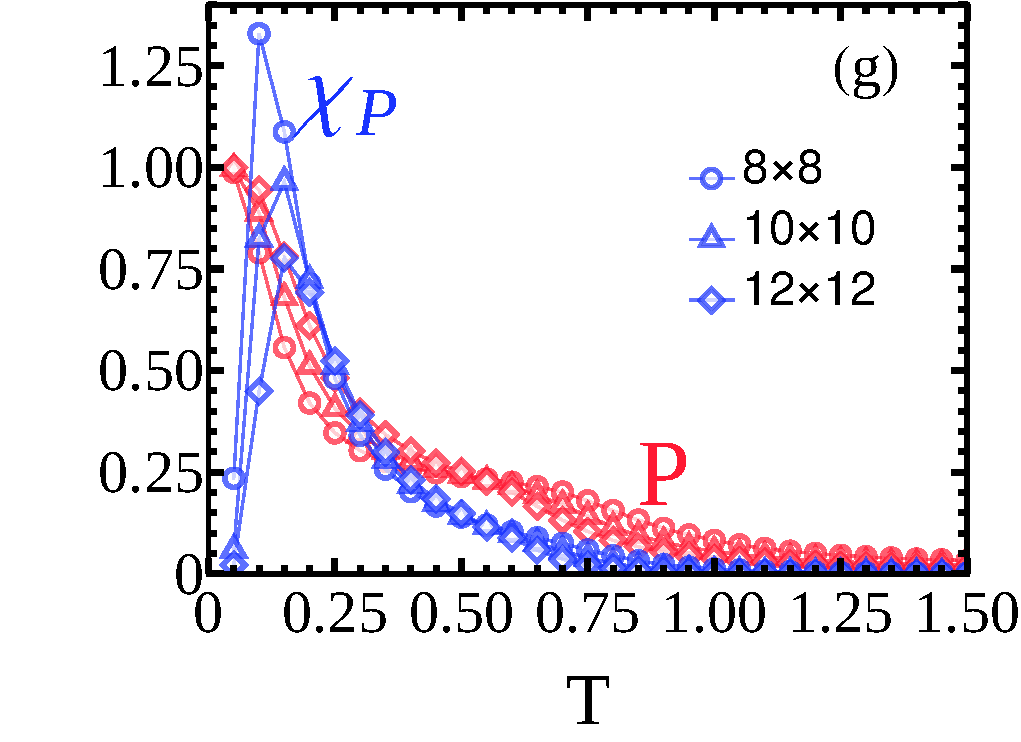
\includegraphics[width=0.32\textwidth]{figures/DIS1.pdf}
%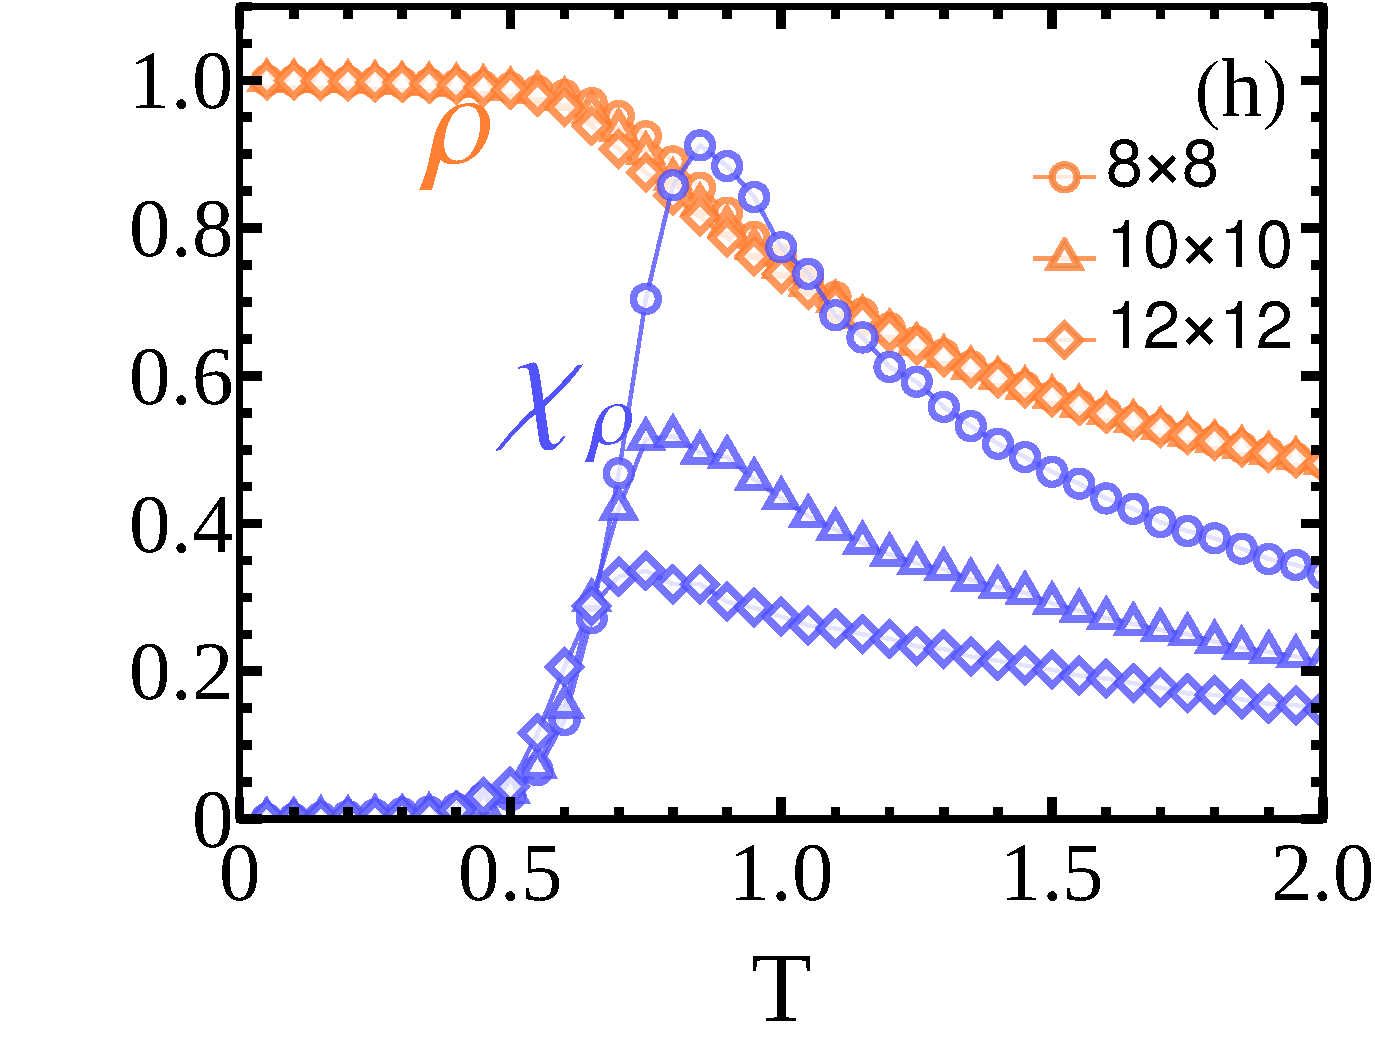
\includegraphics[width=0.3\textwidth]{figures/DIS2.pdf}
%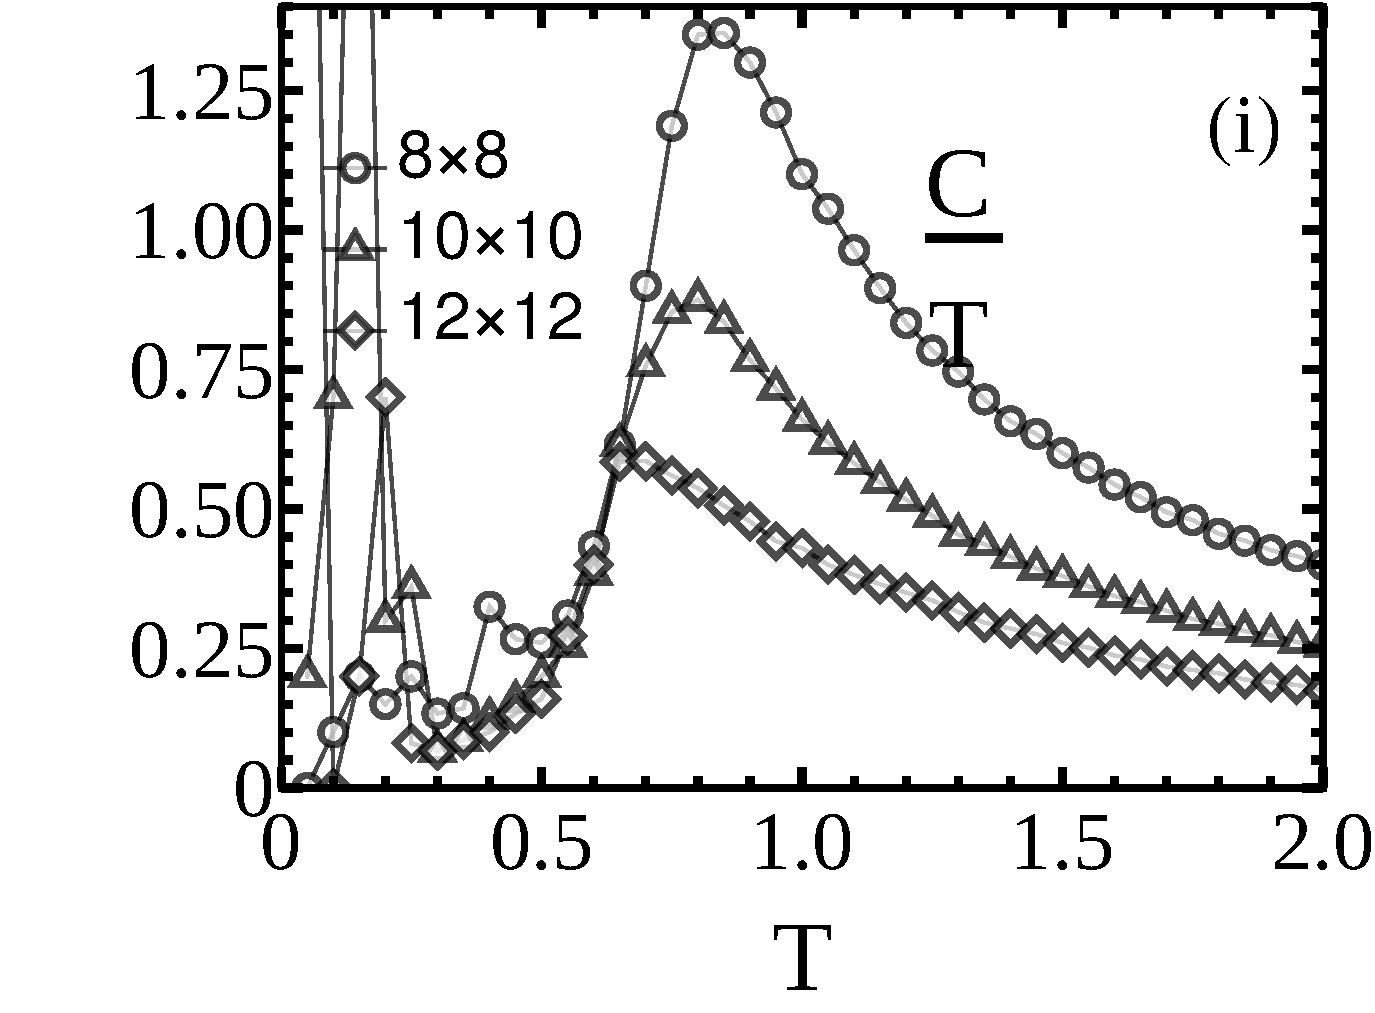
\includegraphics[width=0.31\textwidth]{figures/DIS3.pdf}
\caption{The variation of the order parameter $P$ ((a), (e), (i)), the ice-rule detecting parameter $\rho$ ((b), (f), (j)) and their corresponding susceptibilities $\chi_P$ ((a), (e), (i)) and and $\chi_\rho$ ((b), (f), (j)) as a function of temperature (and field) are shown for different lattice dimensions. Similarly, the specific heat over temperature, $C/T$ is shown in (c), (g), (k) panels. Finally, the uniform magnetic susceptibility is shown in (d), (h), (l) correspondingly. The variation of all the parameters are estimated for three cases as labeled along the vertical axis, that is, AFM (antiferromagnet), FM (ferromagnet), Disorder. All the plots include the same, $\theta$, that is, $\theta=\pi/6$. The values used in each of the cases are: $J_1=0.5$, $J_2=0.04$, $J_3=0.4$ with $8$, $10$, $12$ lattice dimensions used along the interlayer axis, while we fix $12\times 12$ as the intralayer dimensions.}\label{order_param}
\label{order_param}
\end{figure*}
\begin{figure}[t!]
\centering
%\hspace{-1.5cm}
%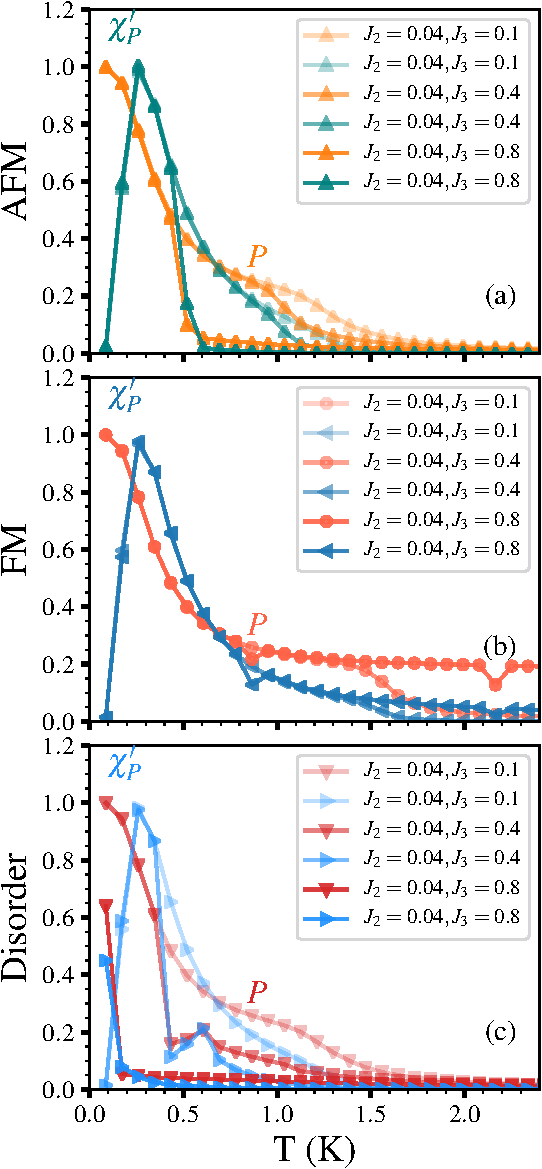
\includegraphics[width=0.40\textwidth]{figures/ice_param.pdf}
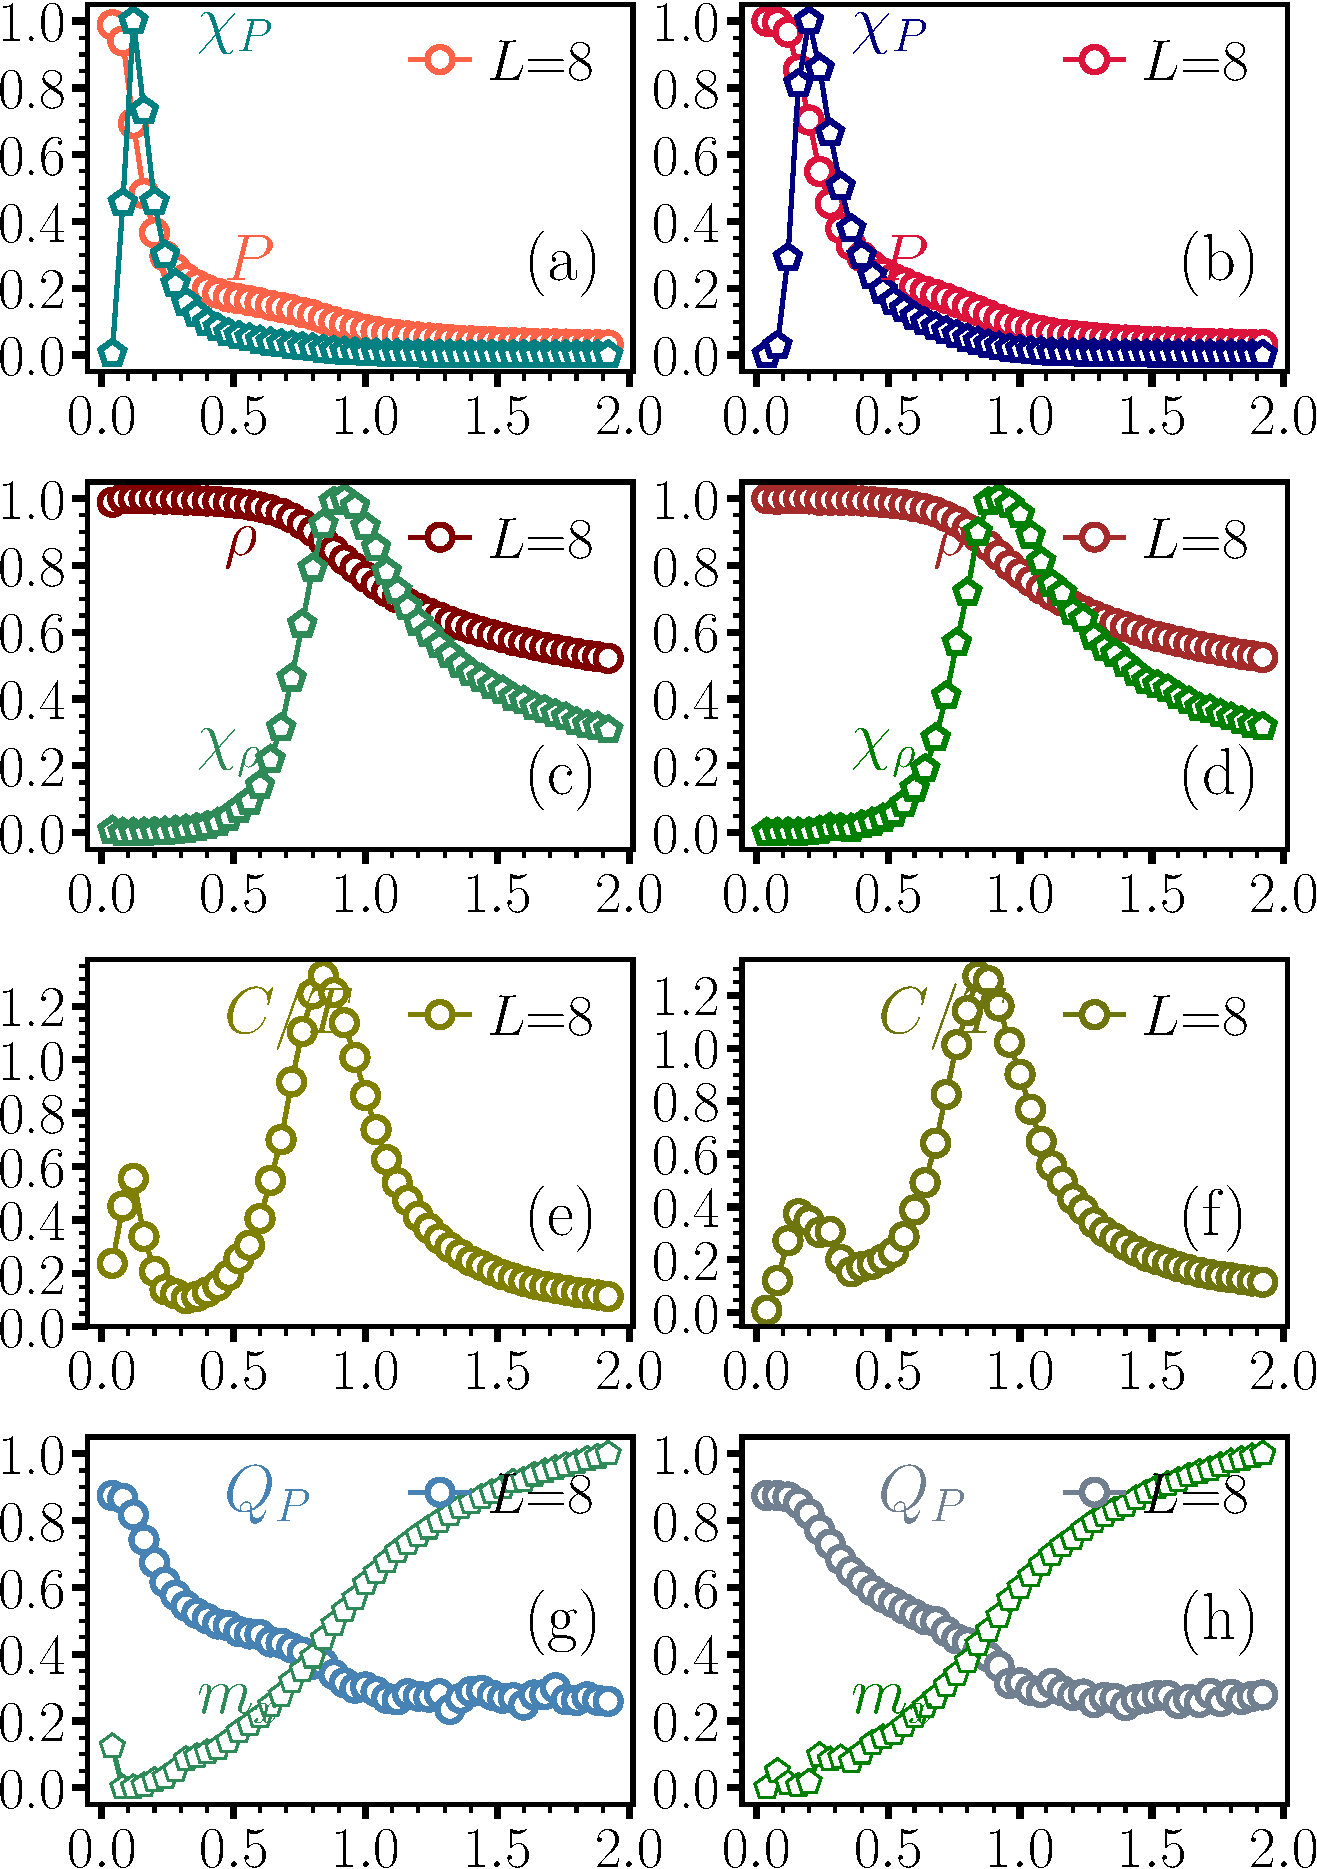
\includegraphics[width=0.48\textwidth]{figures/AFM_TF_0.5_0.03_0_8_16.pdf}
%\includegraphics[width=9.5cm,height=15.0cm,left]{corr_plot_.pdf}
\caption{(Color Online) Variation of the order parameter $P$ and the ice-rule parameter $\rho$ versus field (temperature) are shown for different cases of $J_3$. The interlayer coupling values used are $J_3=0.1,0.4,0.8$ in the increasing trend of the color contrast of respective parameters (e.g: orange color corresponds to $P$ and the increase in $J_3$ can be seen from the least to the highest contrast). a) Corresponds to the variation with AFM, b) FM and c) disordered interlayer couplings}
\label{ice_param}
\end{figure}
\subsubsection{Antiferroelectric phase transition}
%\mandal{Physical reason for choosing the parameter value for $J_3$ and $D$ (We should represent $D$ by $\delta$). It seems sometimes $D$ is greater than $J_3$. Ideally, it should be 10 or 20 percent of $J_3$.}
\indent \indent \textit{Antiferromagnet coupling:} In Fig.~\ref{order_param}(a-d) order parameters $P, \rho$ and corresponding susceptibilities $\chi_P, \chi_\rho, C, \chi_s, Q_P$ are plotted against $K$. Note that not only the temperature is varied but also the field as dictated by the relation $K=T\tan\theta$. So, when a certain temperature value is mentioned, it is to be understood that the corresponding temperature value is $K=T\tan\theta$. Here for Fig.~\ref{order_param} $\theta$ is adjusted to $\pi/6$. We see that the $P$ has a maximum value of 1 till the temperature of 0.3, indicating an antiferroelectric order. As the temperature is increased further, the $P$ shows a plateau behavior for intermediate temperatures (around $K$ $\sim 0.2$ to $0.33$) before vanishing to a conventional paraelectric state ($K>1$). The plateau behavior can be identified as an intermediate state with strong quantum fluctuations~\cite{vijigiri2020dipole,ishizuka2011quantum}. This is because the order parameter $P$ gets vanished around these temperatures while the ice-rule parameter $\rho$ continues to show a constant value of $\rho=1$ till the temperatures of $K=1.1$. So the region of temperatures where the $P$ vanishes to the temperature where the value of $\rho$ starts decreasing from 1 should correspond to a state which satisfies ice-rules. Also, these states should carry a zero net dipole-moment (molecular polarization). This is only possible when each plaquette has a finite dipole moment (molecular polarization) but is randomly oriented with respect to the neighboring plaquettes. Similarly, the values for susceptibility, $\chi_P$ also corroborate the same as a peak around $~$0.25 seems to suggest a possible second-order transition at $K_c=1.70(15), 1.85(27), 2.04(35)$ for $J_3=0.2, 0.3, 0.4$ respectively. Note that the scaling of parameters $P,\rho$ shows a uniform behavior as we vary the linear size of the system from $L_x=8$ to $L_x=12$. For $L_x=8$, the plateau is steeper than that for $L_x=$12. This is intuitive, as the higher sizes are understood to have fewer fluctuations with stable configurations. \\
\indent  Specific heat, $C$ (see Fig.~\ref{order_param}(c)), also shows a small anomalous peak similar to the behavior observed with no interlayer coupling. The susceptibility obtained due to $P$ is shown in Fig.~\ref{order_param}(a)
and (b) by light red colored points which shows a jump at the transition from ferroelectric phase to quantum liquid-like states. This suggests that ferroelectricity is almost destroyed at this transition. However the susceptibility corresponding to $\rho$, that is. $\chi_\rho$ is initially at lower temperatures it is almost zero, which gradually increases until the temperature reaches near the transition from quantum liquid-like states to the paraelectric states. At this transition the $\chi_\rho$ jumps at a higher value and remain almost constant up to a certain temperature which we call $T_{\chi_\rho}$ and after this, $\chi_\rho$ decreases monotonically. The specific heat at a very large temperature shows monotonically decreasing behavior characteristic to the usual paraelectric phase but at low temperature, it shows two peaks of different magnitude as seen in Fig.~\ref{order_param}(c). The largest peak appears at the transition of quantum liquid-like state and we denote this temperature by $T^\star_{C/T}$
. However, the sharp nature of the peak indicates a possible order-disorder phenomenon where the degeneracy seems to be uplifted to some extent. Below this
temperature specific heat shows another small peak at where the $P$ starts to decrease from the initial constant value for small $T$.   This may be
attributed to the fact that the increase of $K$ results in more quantum fluctuations. \\
\indent  In Fig.~\ref{order_param}(d), we plot the results for uniform susceptibility averaged over a single layer show an antiferromagnetic-like order along the orthogonal unit axes spanning the lattice. This shows that as the system size increases the peak height reduces and only vanishes in the thermodynamic limit.     \\
\indent \textit{Ferromagnet coupling:} Similar to the AFM case, the results are shown accordingly in Fig.~\ref{order_param}(e-h). Here also the order parameter $P$ shows a value close to 1 at low temperatures (and temperatures) indicating an antiferroelectric phase. But unlike the AFM case, as we increase the temperatures further the intermediate liquid-like state seems to extend to much larger temperatures compared to the AFM case, indeed the intermediate-liquid-like extends from values of $~0.3$ to $~1.2$. This can be understood that because of FM type coupling, one expects a lesser amount of quantum fluctuations (compared to AFM and disordered case) across the interlayers. This trend is followed similarly by susceptibility since it shows a peak around the same value of $K$ around $~0.25$. This is because we have used the same values of interlayer strength with just opposite signs and thus the peak around the same temperatures. \\
\indent Specific heat curves plotted in Fig.~\ref{order_param}(g) show that cross-over temperatures have slightly shifted to higher temperature values compared to the AFM case (see Fig.~\ref{order_param}(c)). This is in favor of the finding that the intermediate state extends to much larger temperatures in the curves of order parameter $P$. The common aspect in AFM and FM case is about the peak at low temperatures ($\sim 0.3$).
The peak values are the same in both cases, unlike the peak appearing at higher temperatures. Which for the FM case is sharper than the AFM case. This may seem to suggest that a possible order-disorder phenomenon taking place driven by thermal energy. \\
\indent \textit{Disordered coupling:} In this case, we see that $P$ shows a behavior that is very close to the AFM and unlike the FM case. The only difference that we see is in the specific heat curves. We observe that the anomalous peak almost vanishes and also the crossover peak at later temperatures gets broader than the rest of the two cases. This strongly suggests that the disorder completely lifts the degeneracy and there is no re-entrance of the intermediate-liquid-like as such. The values of the specific heat curves are intermediate to that of AFM and FM. In all the cases, the variation of $\chi_s$ is antiferromagnetic. Though for the disorder the antiferromagnetic nature is slightly perturbed (see Fig.~\ref{order_param}(i-l)).\\
\subsubsection{Variation with the interlayer interaction strength}
\indent \indent \textit{Antiferromagnet coupling:} We also plot the behavior of $P$ and  $\rho$ for various values of $J_3$. In Fig.~\ref{ice_param}(a), we have shown the variation of $\chi_P$ and $\chi_\rho$ for $J_3$=($0.1,0.4,0.8$) in orange and navy blue colored points respectively. For large values of $J_3=0.8$, $P$ and $\rho$ have sharper peaks and decrease more rapidly compared to the case of small values of $J_3$. This could be due to the lowered stability of the intermediate liquid-like state as the coupling strength $J_3$ is increased. Also, though the plateau is diminishing, the value of $P$ at low temperatures remains the same for all the cases of coupling. The AFE phase under the AFM type coupling is stable while for the intermediate liquid-like state this is not the case. \\
\begin{figure*}[t!]
\centering
%\hspace{-1.5cm}
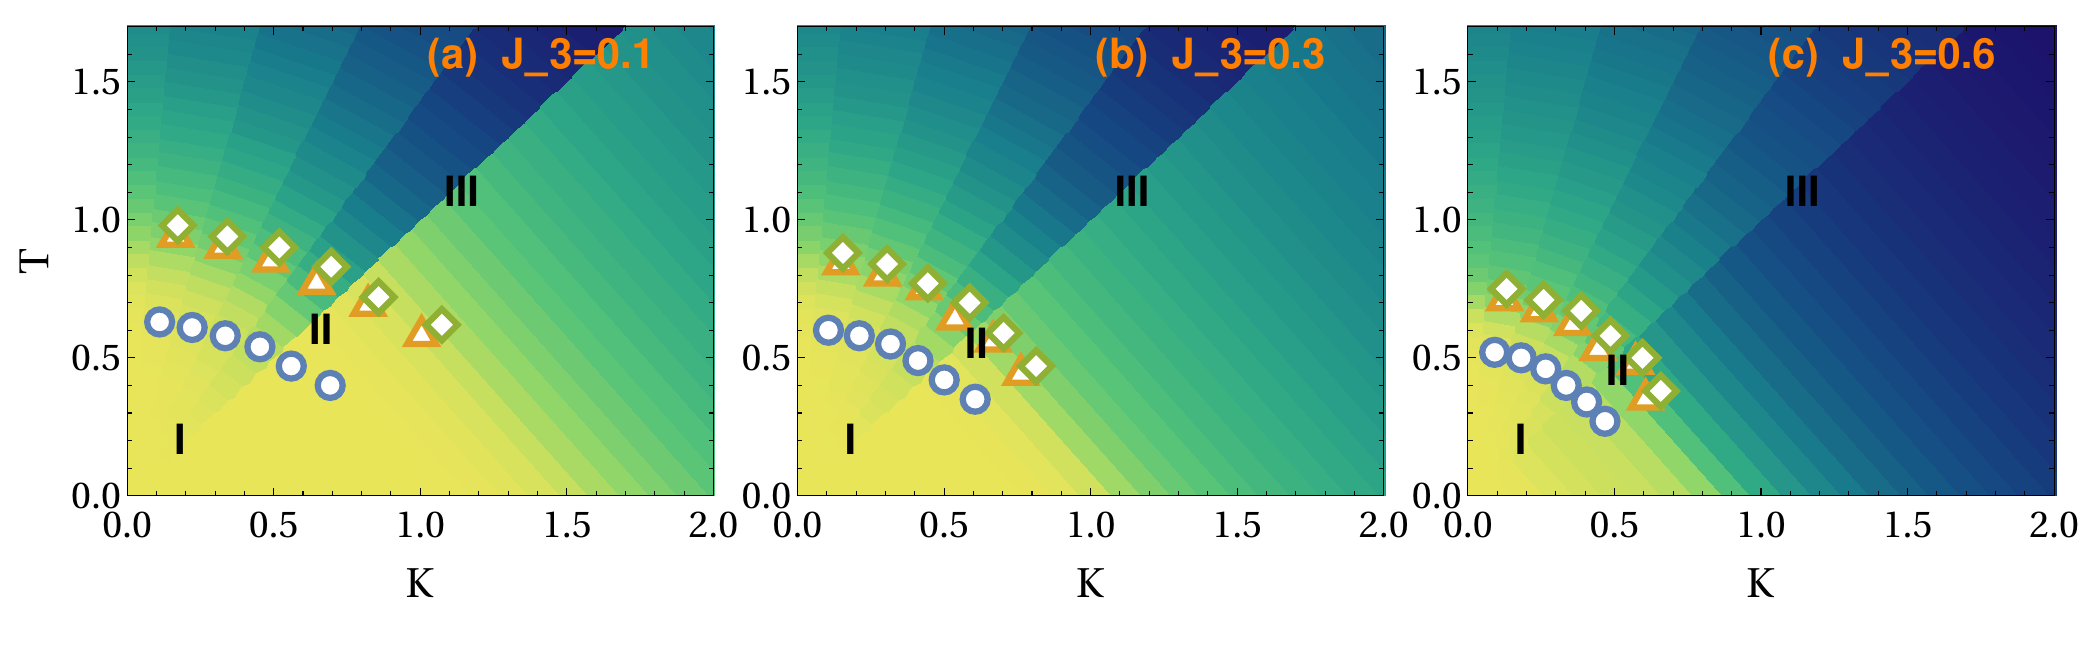
\includegraphics[width=1.0\textwidth]{figures/AFM_phase_diagram.png}
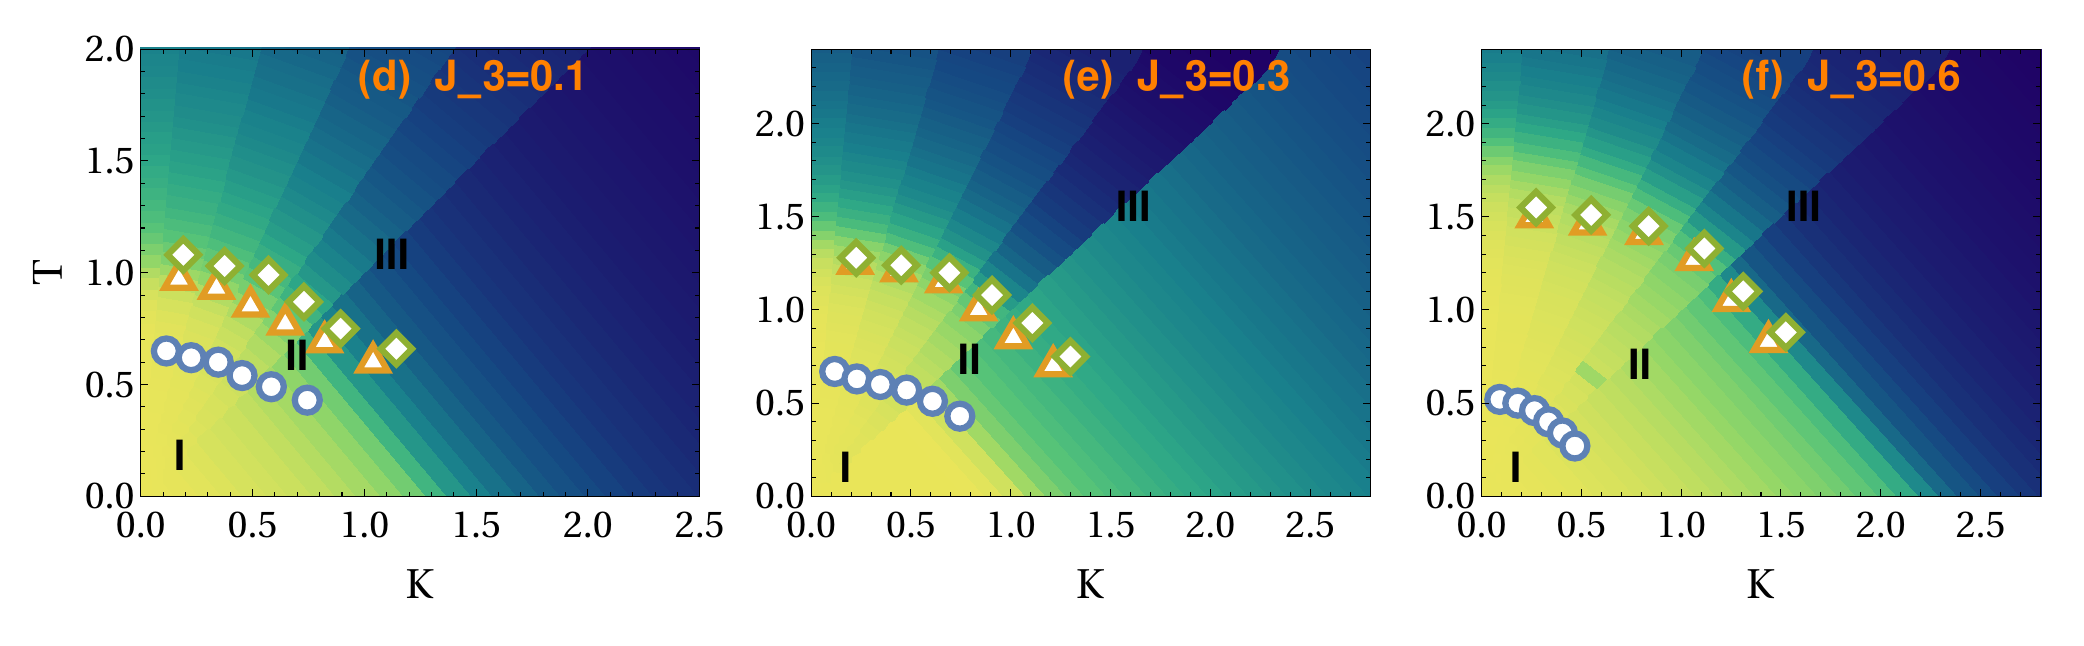
\includegraphics[width=1.0\textwidth]{figures/FM_phase_diagram.png}
%\includegraphics[width=9.5cm,height=15.0cm,left]{corr_plot_.pdf}
\caption{Phase diagram in $T_K$ plane for both the cases, that is, AFM (Fig.~(a)-(c)) and similarly for FM (Fig.~(d)-(f)). In each row starting from the left (Fig.~(a)), the cases correspond to $J_3=0.1,0.3,0.6$ of interlayer coupling strength. The labels \textbf{I}, \textbf{II}, \textbf{III} indicate the AFE phase, Intermediate liquid-like phase and conventional paraelectric phase respectively.}
\label{phase_diagram}
\end{figure*}
\indent \textit{Ferromagnet coupling:} In the Fig.~\ref{ice_param}(b), clearly the plateau region in order parameter $P$ extends to much larger temperatures as the coupling is increased. This is in contrast to the AFM case. When the value of $J_3$ is equal to 0.1, the intermediate liquid-like state extends from $T=0.42$ to $T=0.94$. When $J_3= 0.4$, it extends from $T=0.45$ to $T=1.4$. And for $J_3=0.8$, it is much higher. The reason could be because of the lesser quantum fluctuations in the FM case. Nevertheless, the order parameter $P$ still shows a value of 1 for all the values of coupling strength, $J_3$. This is similar to the AFM case.\\
\indent \textit{Disordered coupling:} In the Fig.~\ref{ice_param}(c), when the value of $J_3$ is small, i.e, 0.1, the variation of order parameter resembles slightly that of AFM and FM case. The plateau region extends from $T=0.25$ to $T=0.75$. But when $J_3$ is increased to $0.4$, we see that the intermediate liquid-like state only extends from $T=0.25$ to $0.6$. Similarly, when $J_3=0.8$, comparable to the energies of the intraplane interactions, the order parameter $P$ has a lower value at lower temperatures. Also, there is no plateau behavior, instead, the abrupt vanishing of $P$ is seen. This could be understood because of more quantum fluctuations induced by disorder type. However, for lower values of interlayer coupling, even the disordered type coupling hosts both an AFE and intermediate liquid-like state. The variation of ice-rule parameter $\rho$ is used to show that there exists an intermediate state with finite-molecular polarization since the value of $\rho$ close to $~$1 indicates that the entire lattice is in an ice-rule state (apart from statistical fluctuations) and any deviation from it indicates a non-ice-rule state. \\
\begin{figure*}[t!]
\centering
\hspace{-0.5cm}
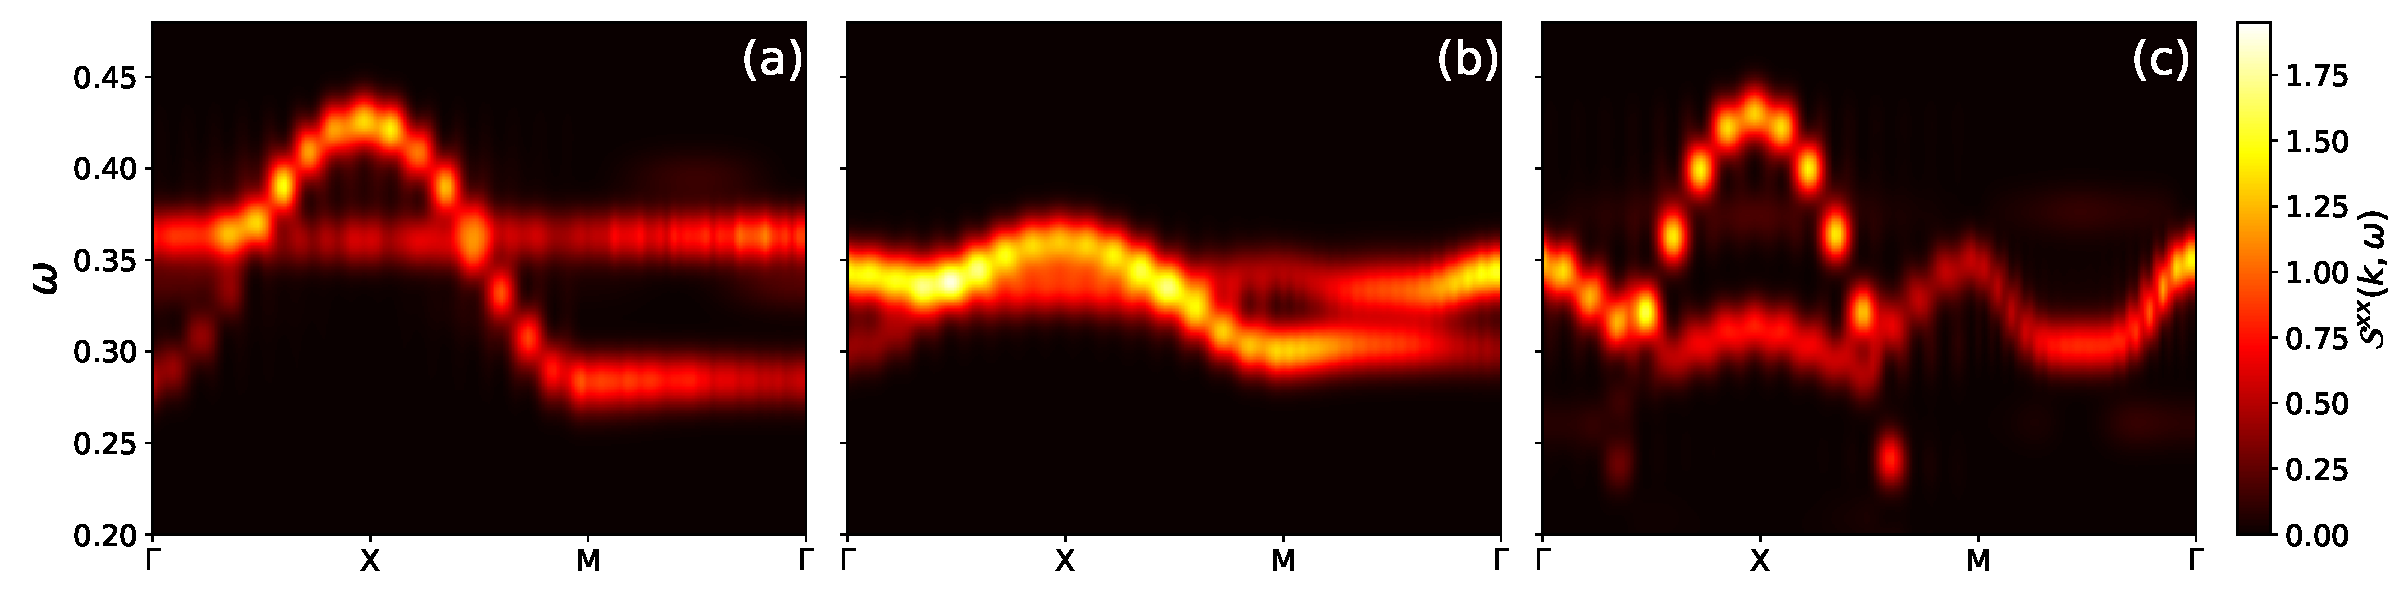
\includegraphics[width=18.0cm,height=4.9cm]{figures/density_plot.pdf}
\caption{The dynamic structure factor, $\mathcal{S}^{xx}(k,\omega)$ within the realm of Real-space linear spin-wave theory (RS-LSWT) calculated for weak interlayer coupling limit. In all the plots, we fix the value of $J_0=1$. a) For the parameters $J_1=1.0$, $J_2=0$, $K_x=0.3$. b) For $J_1=1.0$, $J_2=0.019$, $K_x=0.3$. Similarly, c) For $J_1=1.0$, $J_2=0.3$, $K_x=0.2$. Here, $\Gamma\equiv(0,0)$, $M\equiv(\pi,\pi),X\equiv(0,\pi)$}
\label{density_plot}
\end{figure*}
\subsubsection{Phase diagram}
\indent \indent \textit{Antiferromagnet coupling:} In Fig.~\ref{phase_diagram} (top row), we plot the critical points in the $T-K$ plane as obtained from the the Binder cumulant (see Eq.~\eqref{binder4}). We also plot the peak values of the specific heat curve ($T_{C}$) and the peak in the susceptibility of ice rule order parameter $T_{\chi_\rho}$. For the AFM case, the corresponding values are given in Table~\ref{table}. Clearly, the values the gap between $T_c$ and $T_C$ (or $T_{\chi_\rho}$) is decreasing with the strength of $J_3$.\\
\indent \textit{Ferromagnet coupling:} In Fig.~\ref{phase_diagram} (bottom row), we plot the critical points in the $T-K$ plane as obtained from the the Binder cumulant (see Eq.~\eqref{binder4}). We also plot the peak values of the specific heat curve ($T_{C}$) and the peak in the susceptibility of ice rule order parameter $T_{\chi_\rho}$. For the AFM case, the corresponding values are given in Table~\ref{table}. Clearly, the values the gap between $T_c$ and $T_C$ (or $T_{\chi_\rho}$) is increasing with the strength of $J_3$.
%\begin{figure*}[t!]
%\centering
%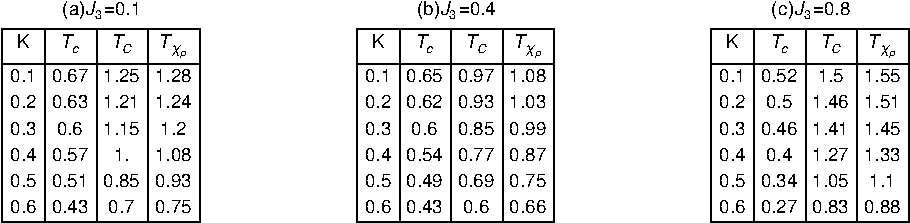
\includegraphics[width=1.0\textwidth]{figures/Values_T.pdf}
%\caption{Table showing the critical points ($T_c$) and the points where the specific heat $C$ and the susceptibility $T_{\chi_\rho}$ peaks. (a) For $J_3=0.1$ value of FM type coupling, (b) for $J_3=0.4$, (c) for $J_3=0.8$. }
%\label{table}
%\end{figure*}
%%%%%%%%%%%%%%%%%%%%%%%%%%%%%%%%%%%%%%%%%%%%%%%%%%%%%%%%
\subsection{Dynamic structure factor}
\label{dynamic}
\indent \indent As mentioned, an earlier study that has not accounted for the interlayer coupling has shown three distinct phases as mentioned~\cite{ishizuka2011quantum,vijigiri2020dipole}. Here, we numerically perform simple linear-spin wave dynamic structure calculations on a real space lattice over the classical ground states of the respective phases identified in a quasi-2D version. We do it on a quasi-2D structure because the interlayer coupling is shown to alter the critical points where the qualitative behavior is not changed. So, the dynamic structure factor can be qualitatively extrapolated from quasi-2D results when an interlayer coupling is introduced for the 3D case. Nevertheless, we note that the present study offers scope to get the low-lying excitations (that can be experimentally tractable) above the classical ground states~\cite{vijigiri2018classical}. Crucial information regarding the degree of fluctuations in the ice-rule physics could also be the best probed to validate certain underlying theories~\cite{chern2014gauge}. We know that in organic ferroelectrics each symmetric arrangement of the molecule posses an associated vibrational mode with it. We, therefore, expect that the amount of frustration mandated by its symmetry can be observed experimentally in the non-resonant Raman-scattering. \\
\indent The brief details on the method and implementation of RS-LSWT are given in Appendix~\ref{RSLSWT}. Fig.~\ref{density_plot} shows the $xx$ dynamical correlation function $S^{xx}(k,\omega)$ plotted for three different regimes under small magnetic fields. In Fig.~\ref{density_plot}(a), we see two bands, one of them is a flat one (no dispersion, see Fig.~\ref{density_plot}(a) at $\omega\sim 0.36(7)$) and the other with a dispersion. The flat band can be understood to be the excitations corresponding to the conserved quantities with a non-local gauge symmetry. Within the linear-spin wave theory probing the excitations under the classical ground states, the gauge operator can be decomposed into non-interacting pairs of correlators, for example, $\sigma^z_1\sigma^z_2\sigma^z_3\sigma^z_4$ $\sim $ $\sigma^{x^\prime}_1\sigma^{x^\prime}_2+\sigma^{x^\prime}_3\sigma^{x^\prime}_4+\cdots$ in the transformed coordinates. Since, for $J_2=0$, the terms $\sigma^x_1\sigma^x_2$ will yield a dispersive term like $\cos k$ and since the further configurations along the unit vectors are independent, we see a $\sin k$ behavior is also likely possible. Therefore, ending with the net result being non-dispersive. Even if one considers a mean-field theory extension to the present scenario we might still see a similar flat band, because these terms do not vanish. Note that the minimum of the spectrum is at multiple $k$-points, i.e, $\omega\sim 0.28$ from $M$ to $\Gamma$ points. This could also reflect the underlying symmetry in the system.\\
\indent Similarly, the optical mode that we see from $\Gamma$ to $X$ and $X$ to $M$ in Fig.~\ref{density_plot}(a) could be associated to the excitations of the correlators of the form $\sigma^{x^\prime}_1\sigma^{x^\prime}_2+\sigma^{x^\prime}_3\sigma^{x^\prime}_4+\cdots$ coming from the gauge operators and as well as the intramolecular interaction term. The decomposition can be understood like all the possible dimer coverings on a plaquette spanning the entire lattice. So then the excitations should correspond to these dimers. Now the reason for the appearance of the optical mode can be understood from ice-rule constraint. Since the configurations along the unit vector that spans the lattice are not completely independent. We expect that the net superposition of the spin-waves should be non-dispersive. That is why we see optical modes when only one component is varied ($k_x$ from $\Gamma$ to $X$ or $k_y$ from $X$ to $M$). But when both the components are varied we see that the net result is flat (from $M$ to $\Gamma$). When $J_2$ is turned on, due to the global ordering being established, we see that the excitations of these dimer coverings have a definite spectrum of the form $\cos k_x$ or $\sin k_y$. We thus see no flat band behavior in Fig.~\ref{density_plot}(a). \\
